\documentclass{hmcthesis}

%%% Other packages needed by your document may be loaded here.
\usepackage{url}              % For formatting URLs and other web or
                              % file references.
\usepackage{mflogo}           % Provides the METAFONT logo.
\usepackage{booktabs}         % Publication-quality tables.
\usepackage{natbib}           % Provides some nice citation and
                              % bibliography formatting commands.
\bibpunct[:~]{(}{)}{;}{a}{,}{,~} % Set some defaults for bibliographic
                                 % punctuation used by natbib.sty.
\usepackage{verbatim}
\usepackage{graphicx}
\usepackage{calc}
\usepackage{subfig}
\usepackage{tabulary}
\usepackage{textcomp}
\usepackage{amsmath}
\usepackage[table]{xcolor}
\definecolor{lightgray}{gray}{0.9}
\usepackage[plainpages=false,pdfpagelabels]{hyperref}

\includeonly{%
%%% Chapter 1
introduction
%%% Chapter 2
,structured-writing
%%% Chapter 3
,mathematics
%%% Chapter 4
,figs-and-tables
%%% Chapter 5
,typesetting
%%% Chapter 6
,tips-and-tricks
%%% Chapter 7
,resources
%%% Chapter 8
,books
%%% Appendix
,versions
}


\setcounter{errorcontextlines}{1000}

\title{Immunospecific Gold Nanoparticles for Contrast Enhancement of Corneal Tissue Culture}

\author{Theodore DuBose}

\advisor{Richard C. Haskell}

\department{Physics}

%\reader{Second Reader}

%% The year in which you are submitting your thesis.
\thesisyear{2012}
                                                                               
\newcommand{\bslash}{\symbol{'134}}%backslash
\newcommand{\bsl}{{\texttt{\bslash}}}
\newcommand{\com}[1]{\bsl\texttt{#1}\xspace}
\newcommand{\file}[1]{\texttt{#1}\xspace}

\newcommand{\pdftex}{PDF\tex}
\newcommand{\pdflatex}{PDF\latex}
\newcommand{\acronym}[1]{\textsc{#1}\xspace}
\newcommand{\key}[1]{\textsf{\emph{#1}}\xspace}
\newcommand{\class}[1]{\textsf{#1}\xspace}
\newcommand{\package}[1]{\textsf{#1}\xspace}
\newcommand{\env}[1]{\texttt{#1}\xspace}
\newcommand{\prog}[1]{\texttt{#1}\xspace}
\newcommand{\command}[1]{\texttt{\bsl{}#1}\xspace}
\newcommand{\ctt}{\texttt{comp.text.tex}\xspace}
\newcommand{\tex}{\TeX\xspace}
\newcommand{\latex}{\LaTeX\xspace}
\newcommand{\host}[1]{\textsf{#1}\xspace}
                                                                               
\newcounter{cms}

%%% Some theorem-like command definitions.

%%% The \newtheorem command comes from the amsthm package.  That
%%% package is loaded by the class file.

\newtheorem{thm}{Theorem}[chapter]
\newtheorem{Theo1}{Theorem}[chapter]
\newtheorem{Theo2}{Theorem}[chapter]
\newtheorem{Lemma}{Lemma}[chapter]


%%% If you find that some words in your document are being hyphenated
%%% incorrectly, you can specify the correct hyphenation using the
%%% \hyphenation command.  Note that words are separated by
%%% whitespace, as shown below.

\hyphenation{ap-pen-dix wer-ther-i-an}


%%% The start of the document!

%% The document environment is the main environment in any LaTeX
%% document.  It contains other environments, as well as your text.

\begin{document}

%%% The front matter of a large document includes the title page or
%%% pages, tables of contents, lists of figures or tables, and so on,
%%% your abstract, a preface or introduction, and so on.  It's
%%% delineated with the \frontmatter command.
\frontmatter

%%% One of the things that the \frontmatter does is make page
%%% numbers appear as lowercase Roman numerals---i, vi, xii, and so
%%% on.

%%% The first thing in the front matter is your title page.  The title
%%% page is formatted by commands in the document class file, so you
%%% don't need to worry about what it looks like -- just putting the
%%% \maketitle command in your document (and filling in the necessary
%%% information for the identification commands above) is enough.
\maketitle


%%% Abstract

%%% Your abstract should be a \emph{brief} summary of the contents
%%% of your report.  Don't go into excruciating detail
%%% here---there's plenty of room for that later.

\begin{abstract}

\end{abstract}


%%% Acknowledgments (Optional).

%%% If you want to thank someone for their influence on your life or
%%% your work, here's where you'd do it.

\begin{acknowledgments}
  
\end{acknowledgments}




%%% Table of Contents, List of Figures, and List of Tables.
%%% 
%%% If you don't have any figures or tables in your report, you can
%%% comment out the appropriate command.

\tableofcontents
\listoffigures
\listoftables
\mainmatter
\chapter{Introduction}
\label{introduction}

According to the National Eye Institute (NEI), approximately 40,000 cornea transplants are performed every year in the United States. Unfortunately, about 20 percent (8000 per year) of these transplants are rejected~\citep{NEIcornea}, necessitating a second transplant. An increase in the number of procedures is inconvenient for the patient at best; therefore, it is desirable to find ways to minimize the amount of rejection as well as increase the overall supply of tissue for cornea transplants.

\section{Corneal Engineering}
\label{cornealengineering}

Prof. Liz Orwin's lab at Harvey Mudd College is attempting to overcome the challenges of cornea transplants by growing replacement corneas. This is done by electrospinning collagen fibers, then seeding cells from a patient who needs new corneas. However, the electrospun collagen does not possess the structural properties of corneal collagen, so the Orwin Lab is focused on finding ways to control the phenotype and regulatory mechanisms of the cells. It is hoped that through this process, the cells will reenact the initial formation of the corneas in fetal development, taking up the electrospun collagen and laying it back down in the native form, viz., a hexagonal close-packed array of 30 nm-diameter collagen fibrils.

In order to better understand the behavior of the cells in response to the treatments they receive, Prof. Orwin's lab would like to be able to monitor both the position and phenotype of the cells in the scaffold. Confocal microscopy, a standard biological imaging modality, has a high ($<1\,\mu$m isotropic) resolution but can only image 25 $\mu$m deep. The high resolution makes confocal desirable, but human corneas are 500 $\mu$m thick, and the collagen scaffolds can be thicker, making confocal unusable for full 3D imaging. In contrast, the optical coherence microscope (OCM) trades high resolution for moderate resolution ($5\,\mu$m lateral, $10\,\mu$m axial) and over 1 mm of depth penetration at 850 nm wavelength. Consequently, the OCM was employed to monitor the cells.

Unfortunately, the collagen in the scaffold scatters too highly for the OCM to distinguish the cells, so Chris Raub '04 proposed a method, developed from a paper by Sokolov~\citep{Sokolov}, wherein 35 nm gold nanoparticles would be applied to increase scattering of the cells via a process called indirect immunolabeling (see \autoref{indirectimmunolabeling})), the basic precepts of which are still used in this project~\citep{raub}. Indirect immunolabeling has four key components: a target protein (we are targeting $\alpha 5 \beta 1$-integrin), a primary antibody (MAB1999) that is \emph{anti}- the target protein, a secondary antibody (AP124F) that is \emph{anti}- the primary antibody, and a label (both the gold nanoparticles and a fluorescent molecule on the AP124F). Indirect immunolabeling is implemented by first binding primary antibodies specifically to their target proteins on the surfaces of corneal cells. Then, secondary antibodies (anti-Ab1) are bound to nanoparticles via van der Waals forces. The antibody-gold is then allowed to bind to the Ab1-protein-cell \emph{in vitro}. A schematic diagram of this process is shown in \autoref{indirectimmunolabeling}.

\begin{figure}[htbp]
\centering
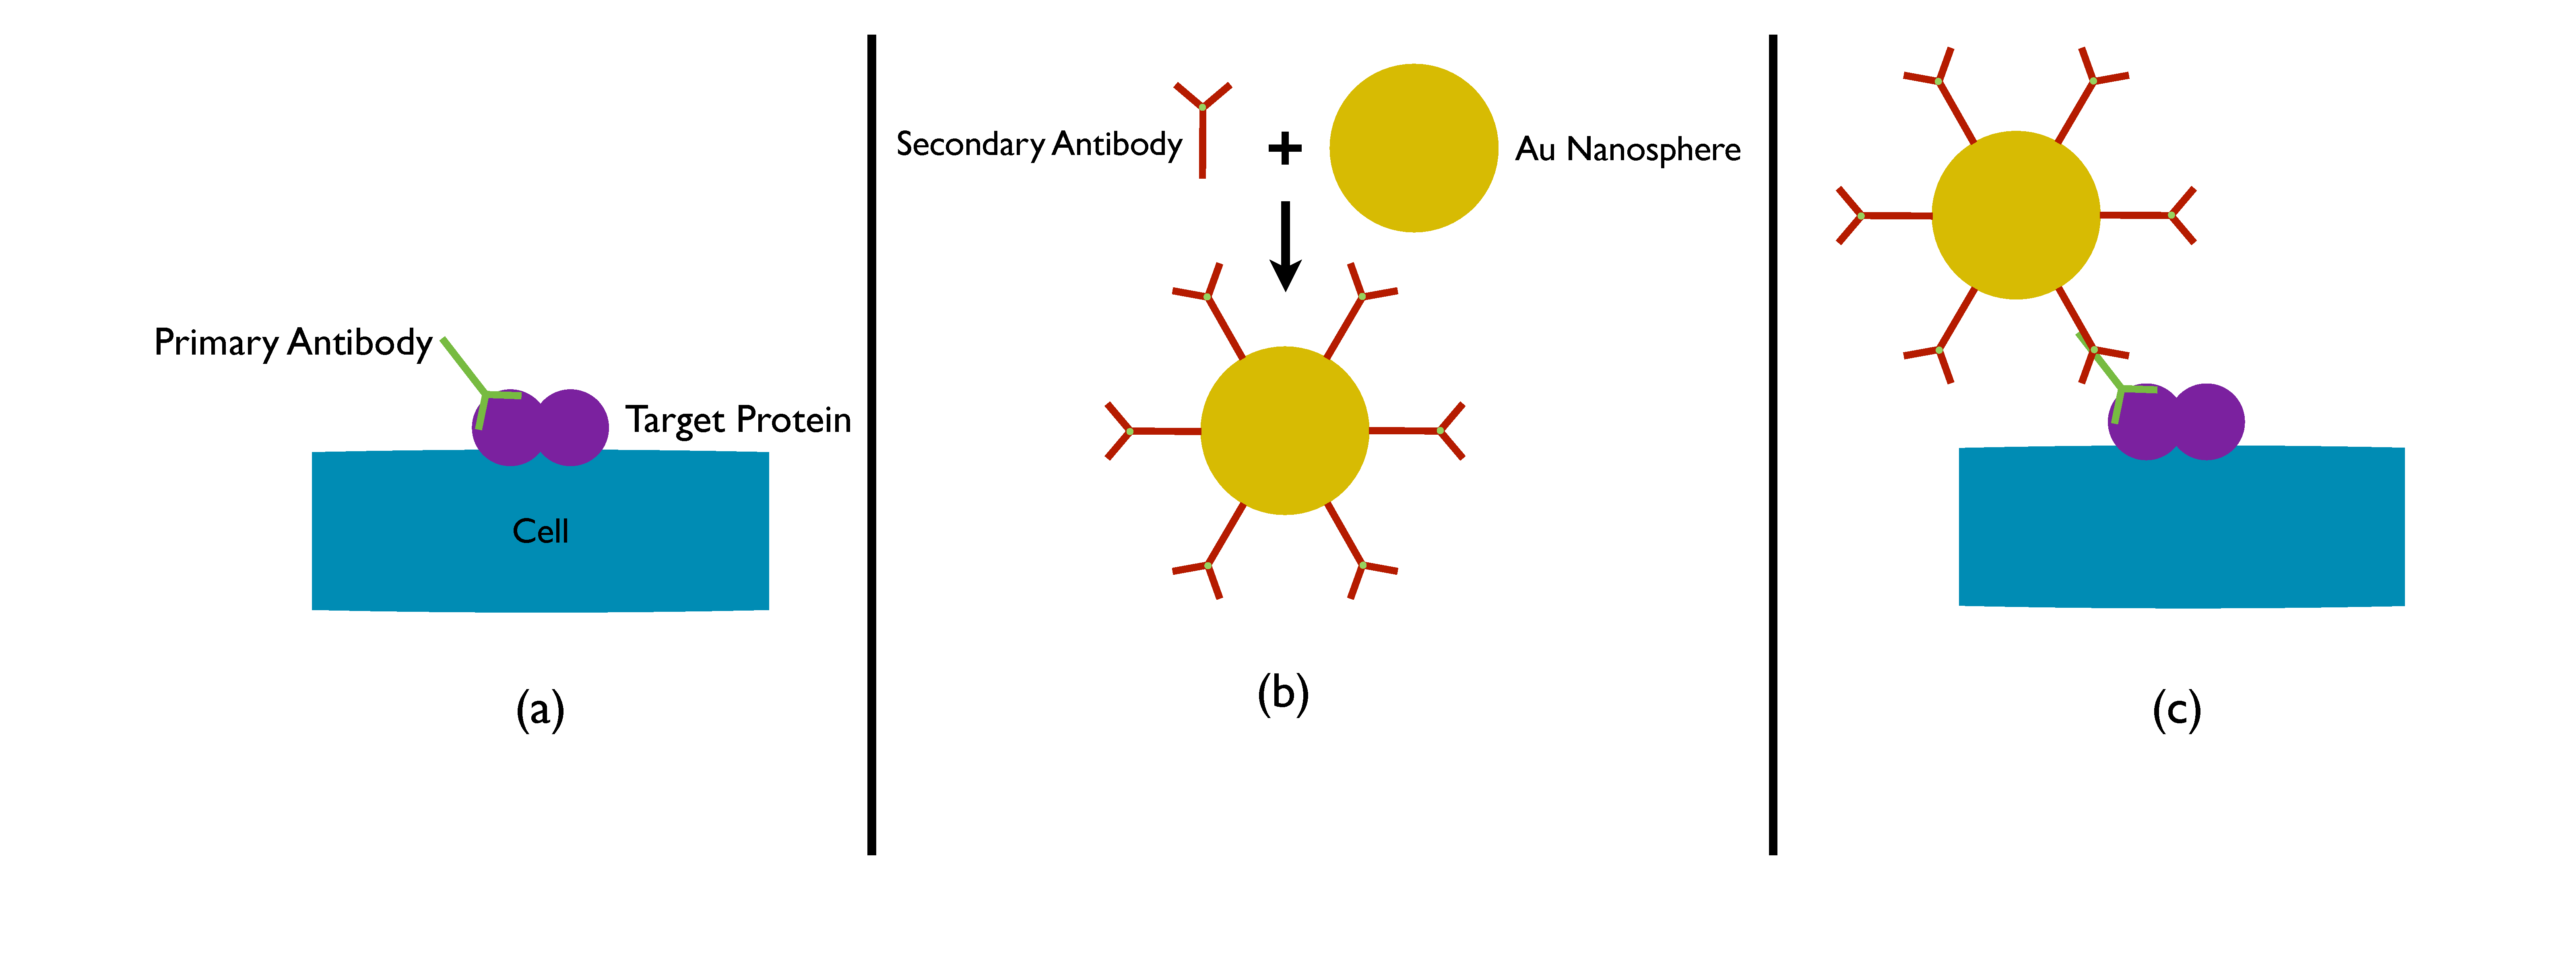
\includegraphics[keepaspectratio,width=\textwidth,height=0.75\textheight]{./IndirectImmunolabeling.pdf}
\caption{Stages of indirect immunolabeling presented schematically (not to scale). (a) The primary antibody, MAB1999, binds to the targeted surface protein, $\alpha 5 \beta 1$-integrin. (b) Secondary antibodies, AP124F, are bound to the surface of a gold nanoparticle. (c) A gold nanoparticle-secondary antibody complex binds to the primary antibody, which is in turn bound to the surface protein.}
\label{indirectimmunolabeling}
\end{figure}



Jamie Shoffeit '05~\citep{chanshoffeit}, Megan Arman '06, and Emily Hogan '07 all followed on Raub's work to achieve labeling. The process they employed consisted of creating 35 nm diameter gold nanoparticles from a citrate reduction of Au(III) and binding the antibodies to the nanoparticles via van der Waals forces alone. Although Hogan was finally able to use this technique to produce a statistically significant increase in scattering in 2007, the scattering increase was not as great as was desired.

To address this, David Coats '08 did a number of studies to optimize the gold being used as the labeling agent. Coats performed extensive calculations using Mie theory to maximize scattering. Mie theory details the scattering pattern of particles on the order of or larger than the wavelength of light they scatter. As even a 35 nm nanoparticle cannot be approximated as a point when using 850 nm light, Mie theory provides a far more accurate prediction of the intensity of backscattered intensity than Rayleigh scattering theory. These calculations showed that for any diameter, a particle made of solid gold (versus a particle with an inner core of silica) gave the highest scattering to absorption cross-section ratio, as shown in \autoref{whatcore}. As can also be seen in that image, $C_{sca}/C_{abs}$ also increases with diameter, up to a point. However, the settling rate of the gold particles also had to be taken into account, as well as the availability of manufactured gold nanoparticles. With these multiple factors in consideration, it was decided that 90 nm diameter nanoparticles from Nanopartz would be used. With these improved gold particles, David Coats again performed imaging tests on a monolayer of cells. However, the same lack of obvious signal generation prompted even further investigation.

\begin{figure}[htbp]
\centering
\includegraphics[keepaspectratio,width=4in,height=0.75\textheight]{CscaCabs.pdf}
\caption{Plot of the ratio of the scattering cross section $C_{sca}$ to the absorption cross section $C_{abs}$ as a function of total particle diameter, calculated via Mie theory. Line color, as indicated by legend, corresponds to percent of total diameter taken up by silica inner core. Index of refraction values used are $n_{\mathrm{Au}}=0.194 - 5.527i$, $n_{\mathrm{silica}}=1.44$, and $n_{\mathrm{water}}=1.33$ for the surrounding region. From reference~\citep{coats}.}
\label{whatcore}
\end{figure}



One concern regarding the labeling system was that the antibodies were bound to the gold with only van der Waals forces. Rob Warren '10~\citep{warren} discovered a procedure in a paper by Lowery et al.~\citep{westpegylation} by which increased binding had been achieved for immunolabeling. The procedure is called PEGylation because of its use of polyethylene glycol polymer chains; a schematic diagram of the process is shown in \autoref{pegylation}. The procedure consists of using a polyethylene glycol (PEG) polymer chain functionalized at one end with orthopyridyl disulfide (OPSS) and at the other with an N-Hydroxysuccinimide ester (NHS). The OPSS-PEG-NHS is incubated with the antibody for 24 hours, in which time the NHS ester reacts with a lysine in the antibody, leaving the NHS ester free in solution and the antibody attached to the OPSS-PEG. This OPAb, as we call it, is then incubated with the gold for 24 hours, so that the OPSS group splits at the disulfide bond and the PEG chain attaches to the gold via a thiol bond, which has a strength slightly less than that of a covalent bond and much larger than that of a van der Waals bond. This should ensure that the antibody is firmly attached to the gold. The second part of the procedure is to prevent any other molecules from binding with the gold. This is accomplished by binding another PEG chain to the gold, of which one end is functionalized with a thiol group (SH) that then forms a thiol bond with the gold. This should fill any space left after the addition of the OPAb. 

\begin{figure}[htbp]
\centering
\includegraphics[keepaspectratio,width=\textwidth,height=0.75\textheight]{PegylationFull.pdf}
\caption{Schematic diagram of the PEGylation process. (a) The OPSS-PEG-NHS (OPN) binds to the antibody (Ab) to form OPAb. (b) The OPAb binds to the Au nanosphere to form OPAb-Au. (c) The PEG-SH fills in the gaps on the surface of the OPAb-Au, forming OPAb-Au-PS and protecting the sphere.}
\label{pegylation}
\end{figure}



Unfortunately, these tests also failed to produce the desired specific increase in scattering, so in the summer of 2010 Oliver Hoidn and Perry Ellis '11 undertook a reexamination of the PEGylation protocol. Several significant results emerged from their studies that indicated problems with the PEGylation protocol. First, the Nanopartz gold nanoparticle solution, though its pH is advertised as between 6 and 8, was actually measured at a pH between 5 and 5.5~\citep{hoidnellis} due to the lack of a buffer in the solution. However, if commercial PBS is added, the salt in that solution screens the negative capping agent on the gold nanoparticles, thus eliminating the mutual repulsion between the nanoparticles and causing them to agglomerate and fall out of solution. To remedy this, a buffer solution made of Na$_2$HPO$_4\cdot$7H$_2$O and NaH$_2$PO$_4\cdot$H$_2$O was added to the gold to achieve a total salt concentration of 10 mM. This concentration was chosen as it provides a sufficient level of buffering without screening the capping agent too much. However, over the course of the several days required for the full PEGylation process, it was found that the final immunolabeled gold nanoparticles still suffered from a high rate of agglomeration. A footnote was then found in Lowery et al.~\citep{westpegylation} that noted that PEG-SH cannot perform its protective function unless it has a molecular weight of at least 5 kDa. As the PEG-SH used up to that point had been of molecular weight 1.2 kDa, it had not protected the gold.

Thus, after Oliver and Perry concluded their work in the summer of 2010, it remained to readjust the PEGylation protocol for 5 kDa PEG-SH, and to use that updated protocol to once again try to significantly increased specific immunolabeling. In addition, it was discovered that the NHS ester used to bind the OPN to the antibody can undergo hydrolysis, rendering it incapable of binding; therefore, it was also necessary to examine the hydrolysis of the NHS ester. To date, the issue of NHS hydrolysis has been settled (\autoref{additionofantibodiestonanospheres}) and the PEGylation protocol has been optimized with the 5 kDa PEG-SH (\autoref{additionofpeg-shtonanospheres}). The optimized protocol produces strucural results consistent with the model of PEGylation we have developed (\autoref{resultsofthefullprotocol}). In addition, the 5 kDa PEG-SH appears to provide excellent long-term protection against agglomeration of the spheres. Spheres made with the optimized protocol have been used in two labeling experiments (\autoref{resultsofthe6marchlabelingsession} and \autoref{resultsofthe3aprillabelingsession}), which have provided further insights into the immunolabeling process.

\newpage
\chapter{Addition of Antibodies to Nanospheres}
\label{additionofantibodiestonanospheres}

At the end of the summer of 2010, Oliver Hoidn and Perry Ellis had determined that the optimal number of OPSS-PEG-antibody (OPAb) molecules per nanosphere was approximately 2000; however, there were significant concerns as to whether the OPSS-PEG-NHS (OPN) was successfully binding to the lysines on the antibody, or whether monolayer formation was simply the result of the antibodies binding to the nanospheres via van der Waals forces. The OPN reaction occurs by substituting the NHS ester for a primary amine, such as the one found on the functional groups of lysines in an antibody. A diagram of this reaction is shown in \autoref{nhsreactionpic}.

\begin{figure}[htbp]
\centering
\includegraphics[keepaspectratio,width=\textwidth,height=0.75\textheight]{NHSreaction.jpg}
\caption{Schematic diagram of the OPN+antibody$\to$OPAb reaction. \textbf{R} represents the OPSS-PEG, and \textbf{R'} represents the antibody. The reaction is favored in basic conditions. From ~\citep{nhsreaction}}
\label{nhsreactionpic}
\end{figure}



OPN comes in a lyophilized form, and the reaction with the antibody does not occur until the OPN is in solution. However, once the OPB is in solution, a competing reaction begins in which hydrolysis occurs and the NHS ester is replaced with a hydroxyl group instead of an amine. This renders the molecule unable to bind to antibodies, and the half-life of the hydrolysis reaction can be on the order of minutes at pH 8~\citep{nhshalflife}. Consequently, there was a concern that a large portion of the OPN used in the OPN+antibody$\to$OPAb reaction was not binding to the antibody.

Fortunately, a direct physical measurement can be used to quantify the hydrolysis of the NHS ester. The free NHS ester in solution absorbs at 260 nm much more strongly than the bound ester~\citep{Miron_Wilchek_1982}. Therefore, the Cary 5000 UV-Vis-IR Spectrophotometer was used to monitor the absorption at 260 nm over the course of several hours. The results of this measurement are shown in \autoref{nmabsorption}.

\begin{figure}[htbp]
\centering
\includegraphics[keepaspectratio,width=4in,height=0.75\textheight]{NHShydro.pdf}
\caption{Plot of the absorbance of the OPN solution over time. The reaction rate seems to be proportional to concentration, giving a simple first-order rate law. The lower density of points at \ensuremath{\sim}80 minutes occurred because the spectrophotometer was set to record a spectrum every 10 minutes rather than every 1 minute. The blue line displays a fit to $A = C_1 + C_2\, e^{-C_3 t}$. The fitted values were $C_1=1.16$, $C_2=-0.458$, and $C_3=0.0052$}
\label{nmabsorption}
\end{figure}



Based on the coefficient of the exponent, $C_3=0.00523\,\mathrm{min^{-1}}$, we can calculate that the half-life of NHS ester hydrolysis at pH 7.5 is \[\tau_{1/2}=\frac{\ln 2}{C_3} = 133\mathrm{\,min}\]
or about two hours.

Two conclusions can be drawn from this: first, there is very little danger of having no bound NHS remaining when the protein is added, since that should occur at the most 10 minutes after the OPN solution is created (and will most likely be less than five minutes after solution creation). Second, this confirms the need to incubate the protein with the OPN overnight. Since both hydrolysis of the NHS and the reaction with the lysine work on a similar mechanism, their rates can be expected to be comparable. Thus, in order to create as much OPAb as possible, at least four hydrolysis half-lives are necessary to achieve $>90\%$ yield. However, since the hydrolysis is nontrivial on that time scale, OPN should be used in a factor of 2 excess in order to facilitate maximal protein binding. Therefore, in the PEGylation procedure, we will use 2,000 antibodies per Au nanosphere and 4,000 OPN molecules per nanosphere (see \autoref{ThePEGylationProtocol}).

\newpage
\chapter{Addition of PEG-SH to Nanospheres}
\label{additionofpeg-shtonanospheres}

With the questions about OPN-to-antibody and OPAb-to-nanosphere binding settled, it still remained to determine the optimal concentration of PEG-SH (PS). The PEG-SH is used expressly for the purpose of protecting the gold nanospheres from agglomerating when placed in a salt solution, e.g. the phosphate-buffered saline (PBS) solution present in a cell culture. However, Ellis and Hoidn found that the 1 kDa PEG-SH used since PEGylation was first introduced~\citep{warren} failed to adequately protect the spheres, leading to a significant degree of agglomeration, as shown in \autoref{protection1kda}. A footnote found by Ellis and Hoidn in Lowery et al.~\citep{westpegylation} noted that PEG-SH with a molecular weight less than 5 kDa does not protect gold, explaining the failure of the 1.2 kDa PEG-SH.

\begin{figure}[htbp]
\centering
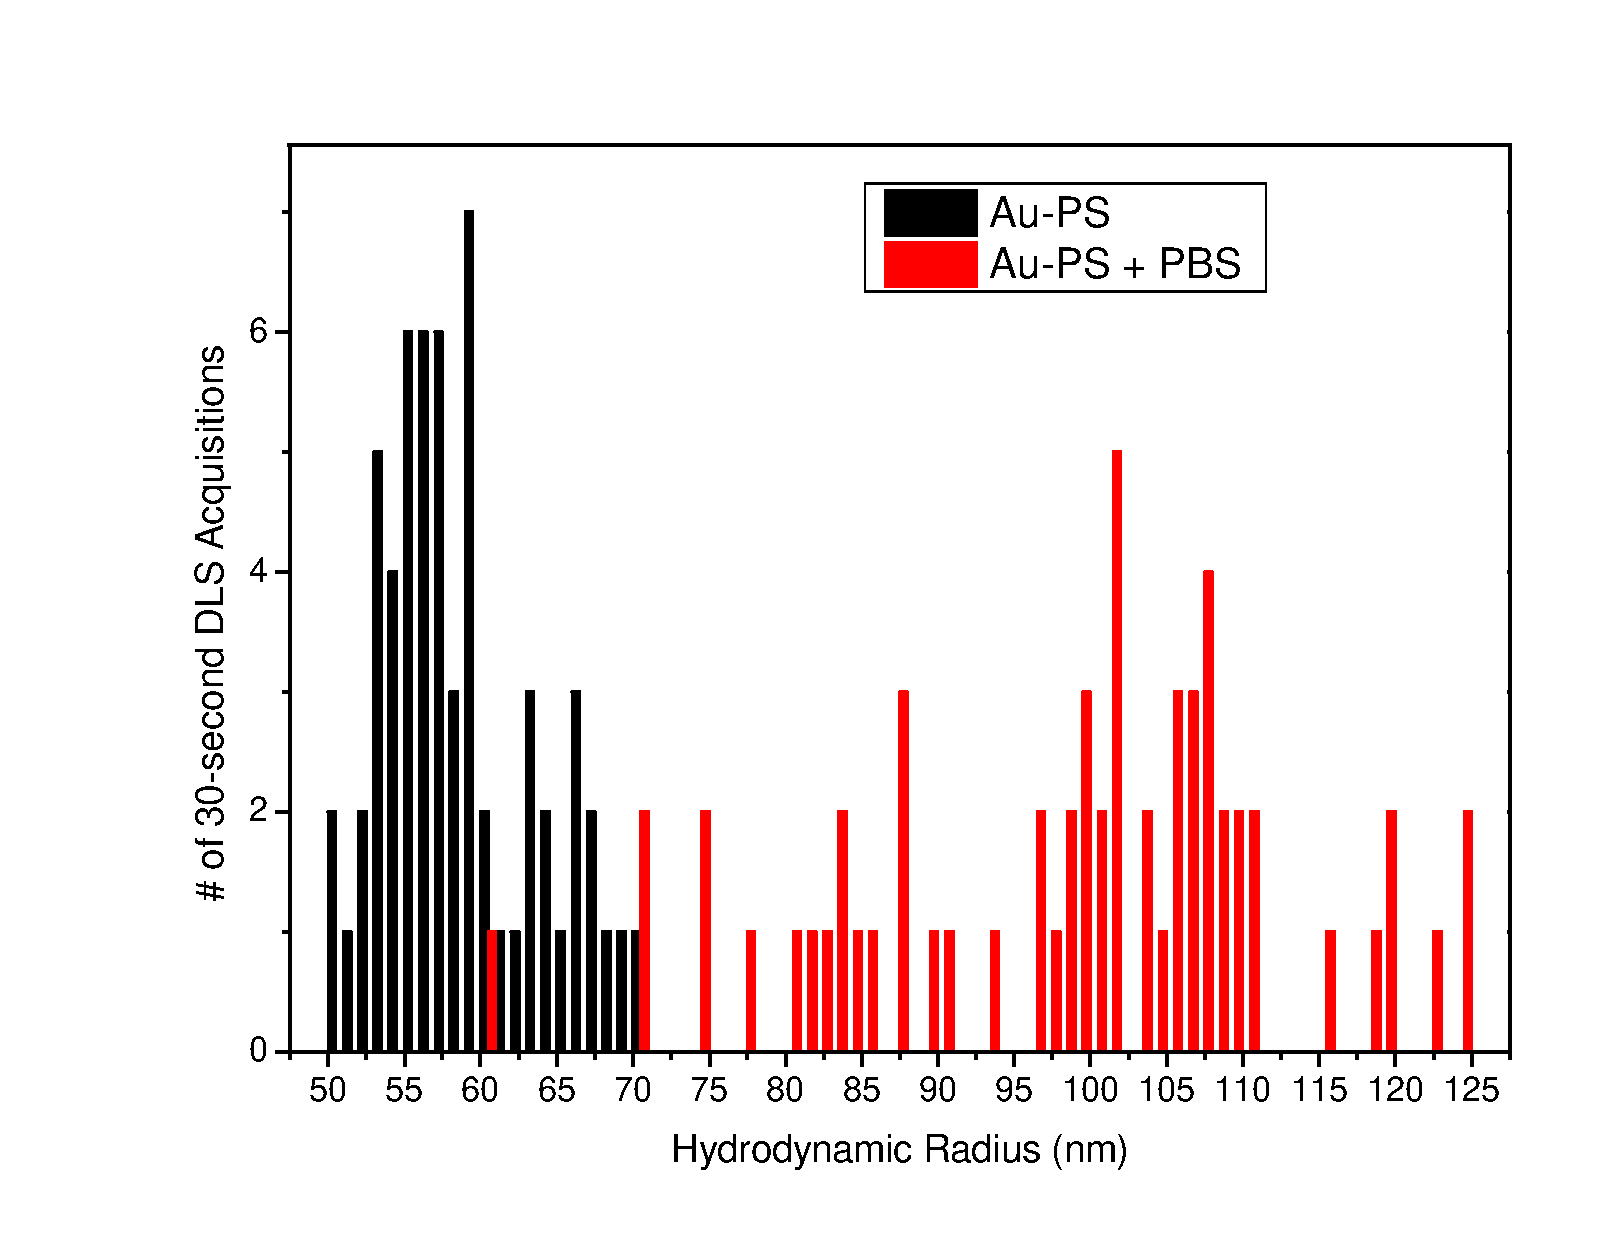
\includegraphics[keepaspectratio,width=4in,height=0.75\textheight]{10^7.pdf}
\caption{Histogram of radii of 30-second DLS acquisitions of $10^7$ 1 kDa PS/Au with and without PBS from the summer of 2010. The distribution is noticeably shifted to the right and flattened after the addition of PBS. Data taken by Ellis and Hoidn~\citep{hoidnellis}.}
\label{protection1kda}
\end{figure}



At the end of the summer of 2010, 5 kDa PEG-SH had not yet been used or characterized, so a completely new optimization process had to be a applied. This consisted of measuring the radii of the gold spheres immediately after the addition of a variety of concentrations of 5 kDa PEG-SH (\autoref{titrationstudy}); measuring the radii of the same solutions after an incubation period (\autoref{timestudy}); and measuring the radii of some solutions after addition of salt solution (\autoref{protectionstudy}). These measurements yielded a monolayer number for 5 kDa PEG-SH of approximately 50,000 PS\slash Au. Strong protection of the nanospheres was also demonstrated at 10,000 PS\slash Au. Therefore, 10,000 PS\slash Au was used as the concentration for the full protocol, as it provides protection, and there should already be a monolayer of OPAb on the surface of the nanospheres.

\section{Titration Study}
\label{titrationstudy}

A titration curve was made by adding 5 kDa PS to 90 nm gold nanospheres (R=52 nm) in varying concentrations, from 1000 PS per nanosphere to $10^7$ PS per nanosphere; the broad range was used to determine the range of concentrations in which the monolayer formed. The hydrodynamic radii of these PEGylated nanospheres were then measured using the Dynamic Light Scattering (DLS) instrument, taking 15 30-second acquisitions of each solution and discarding the first three to account for temperature acclimation. The results of these exploratory measurements are shown in \autoref{kdapegshnewexpl}.

\begin{figure}[htbp]
\centering
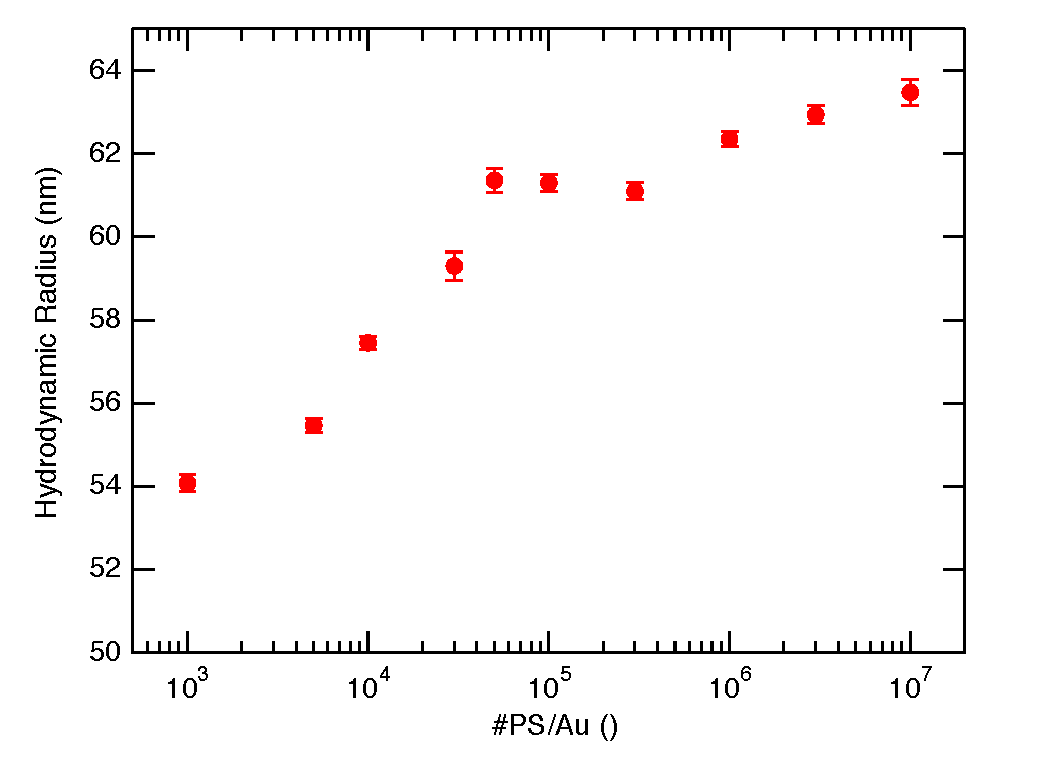
\includegraphics[keepaspectratio,width=\textwidth,height=0.75\textheight]{./ImmediateExploratory.pdf}
\caption{Plot of hydrodynamic radii of Au nanospheres from 1,000 to $10^7$ PS\slash Au less than 30 minutes after addition of PS.}
\label{kdapegshnewexpl}
\end{figure}



This plot shows the behavior of a rapid rise followed by a plateau that is expected of a species forming a monolayer on a surface. The plateau begins to appear around 100,000 \#PS\slash Au, so two more measurements were taken with a spread of concentrations around that range. A plot of the averages of the radii of the repeated concentrations are shown in \autoref{kdapegshnewavg}. This data suggests that the monolayer is formed at approximately 50,000 \#PS\slash Au, with a radius of $60.4\pm0.3$ nm.

\begin{figure}[htbp]
\centering
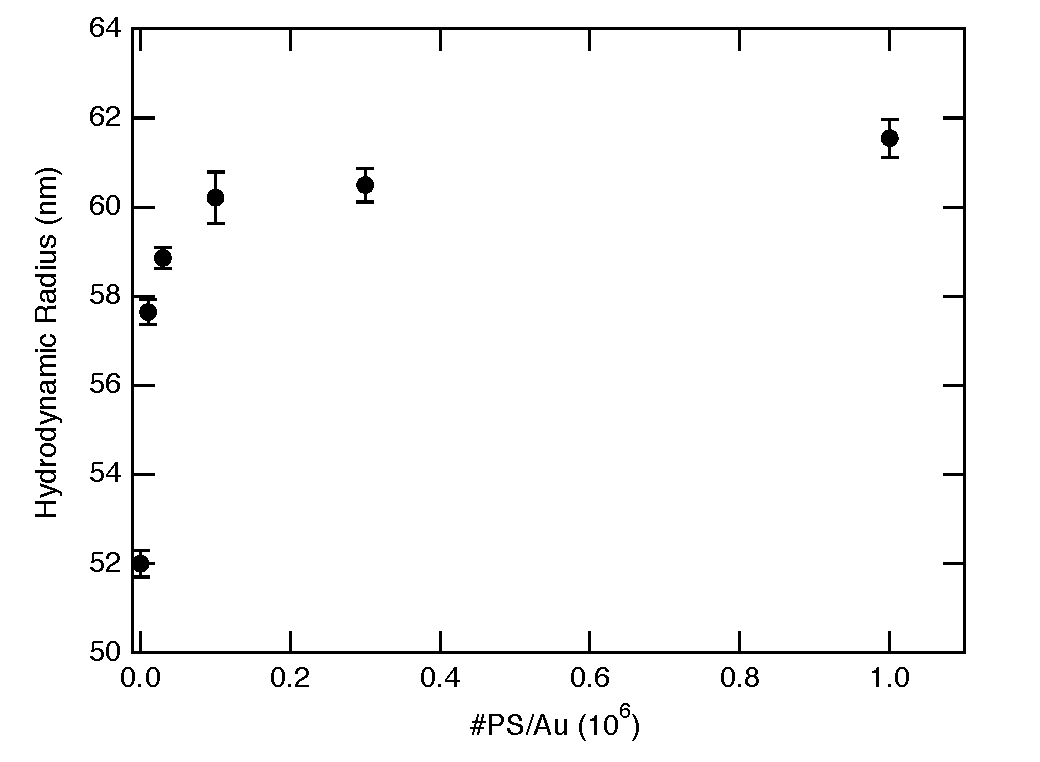
\includegraphics[keepaspectratio,width=\textwidth,height=0.75\textheight]{ImmediateAvg.pdf}
\caption{Plot of hydrodynamic radii of Au nanospheres at 10,000, 30,000, 100,000, 300,000, and $10^6$ PS\slash Au less than 30 minutes after addition of PS. Points are formed by taking the mean and standard error of three independent measurements at each concentration.}
\label{kdapegshnewavg}
\end{figure}



\section{Time Study}
\label{timestudy}

The same samples used in the titration study were measured again after 48--72 hours of incubation, producing the radii shown in \autoref{kdapegshtime}.

\begin{figure}[htbp]
\centering
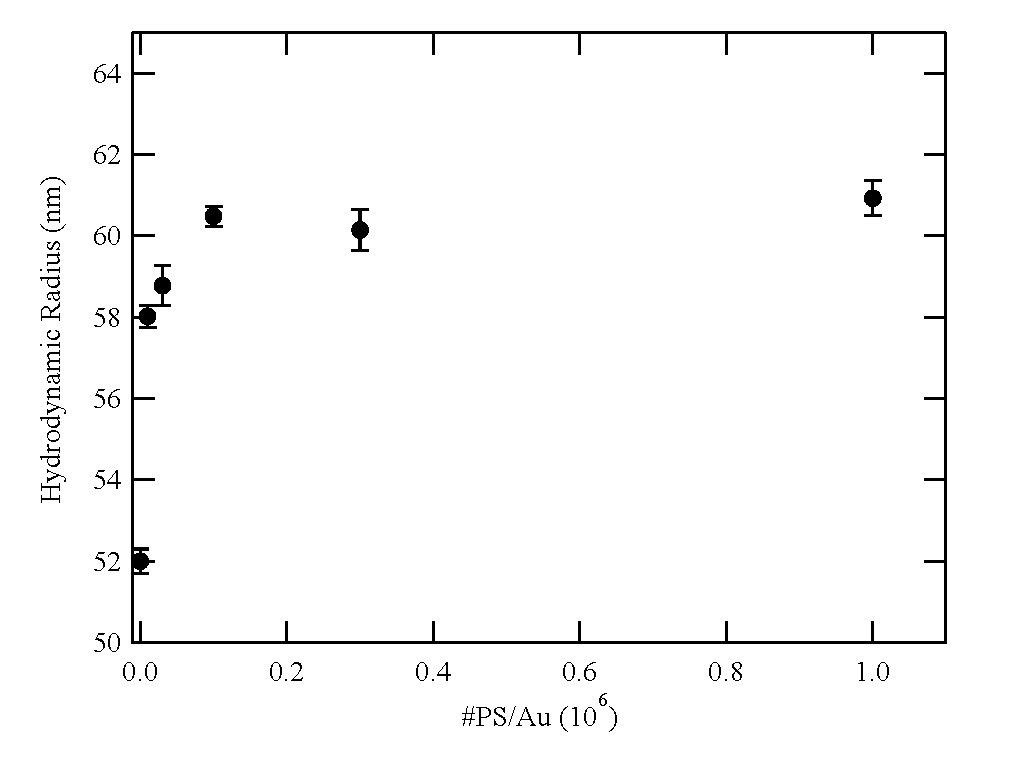
\includegraphics[keepaspectratio,width=\textwidth,height=0.75\textheight]{TimeAvg.pdf}
\caption{Plot of hydrodynamic radius of Au nanospheres at the same concentrations as in \autoref{kdapegshnewavg} 48--72 hours after addition of PS. Points are formed by taking the mean and standard error of three independent measurements at each concentration.}
\label{kdapegshtime}
\end{figure}



The plateau in this graph is slightly sharper than in \autoref{kdapegshnewavg}, indicating that van der Waals forces and thiol bonding processes are in competition, with van der Waals binding dominating immediately after addition, but the lower-energy thiol bonds dominating after incubation time. This leads to the increased radius of the lower-radius samples and the decreased radius of the higher-radius samples. However, the plateau region still has $R=60.3\pm0.3$ nm, as a second indication of a monolayer. Clearly, it is essential that PEG-SH be allowed to incubate with spheres to allow for the PEG-SH binding to reach equilibrium.

More information about the final monolayer state can be gained from determining the apparent number of PEG-SH molecules bound to the nanosphere. A single 5 kDa PEG-SH molecule, with a density of $1.11\,\mathrm{\frac{g}{cm^3}}$, has a volume of
\[\mathrm{V_{5\,kDa\ PEG-SH}}
=\frac{5\mathrm{kDa}}{1.11\frac{\mathrm g}{\mathrm cm^3}}=7.5\mathrm{\,nm^3}\]
This means that a 5 kDa PEG-SH monolayer has, based on the change in hydrodynamic radius,
\[\#_{\mathrm{5\,kDa\ PEG-SH}}=
\frac{\frac{4}{3}\pi((60.5\mathrm{\,nm})^3-(51.0\mathrm{\,nm})^3)} {V_{\mathrm{5\,kDa\ PEG-SH}}}=48,400\pm900\mathrm{\ 5\,kDa\ PEG-SH}\]
This indicates that the measurement of the plateau as beginning at 50,000 PEG-SH per nanosphere is correct. This also allows us to get a sense of the effective footprint of a PEG-SH molecule as it sits on the gold. At monolayer concentration, the area on the surface of the gold taken up by each PEG-SH molecules is
\[A_{\mathrm{PS}}=\frac{4\pi(51.5\mathrm{\,nm})^2/\mathrm{Au}} {47,500\,\mathrm{\frac{PS}{Au}}}=0.70\pm0.03\frac{\mathrm{nm}^2}{\mathrm{PS}}=70\pm3\frac{\text{\AA}^2}{\mathrm{PS}}\]
This size is determined partially by the atomic size of the sulfur atom ($D=2\text{\AA}$), but mostly by the extent to which the PEG chain is bunched; clearly, most of the effective width comes from the bunching.

\section{Protection Study}
\label{protectionstudy}

As mentioned above, the main reason for using 5 kDa PEG-SH is to prevent the Au nanospheres from agglomerating. The Au nanosphere solution includes a negatively charged capping agent that makes the spheres repel each other; when the solution is buffered at pH \ensuremath{\sim}7.5 to prevent antibodies from denaturing during the full immunogold procedure, positive ions are introduced into the solution that neutralize the capping agents, causing the gold nanospheres to agglomerate. Theoretically, PEG-SH would prevent this from happening, but 1 kDa PEG-SH does not, as shown in \autoref{protection1kda}.

Therefore, the protection capabilities of 5 kDa PS were tested by adding PEG-SH to the Au nanospheres in various concentrations, then mixing those solutions in equal volumes with commercial PBS, which has a salt concentration over 100 mM!!. The spheres were allowed to incubate for at least 30 minutes with the PBS, then measured in the DLS. Selected results from those measurements are shown in \autoref{protection}.

\begin{figure}[htbp]
\centering
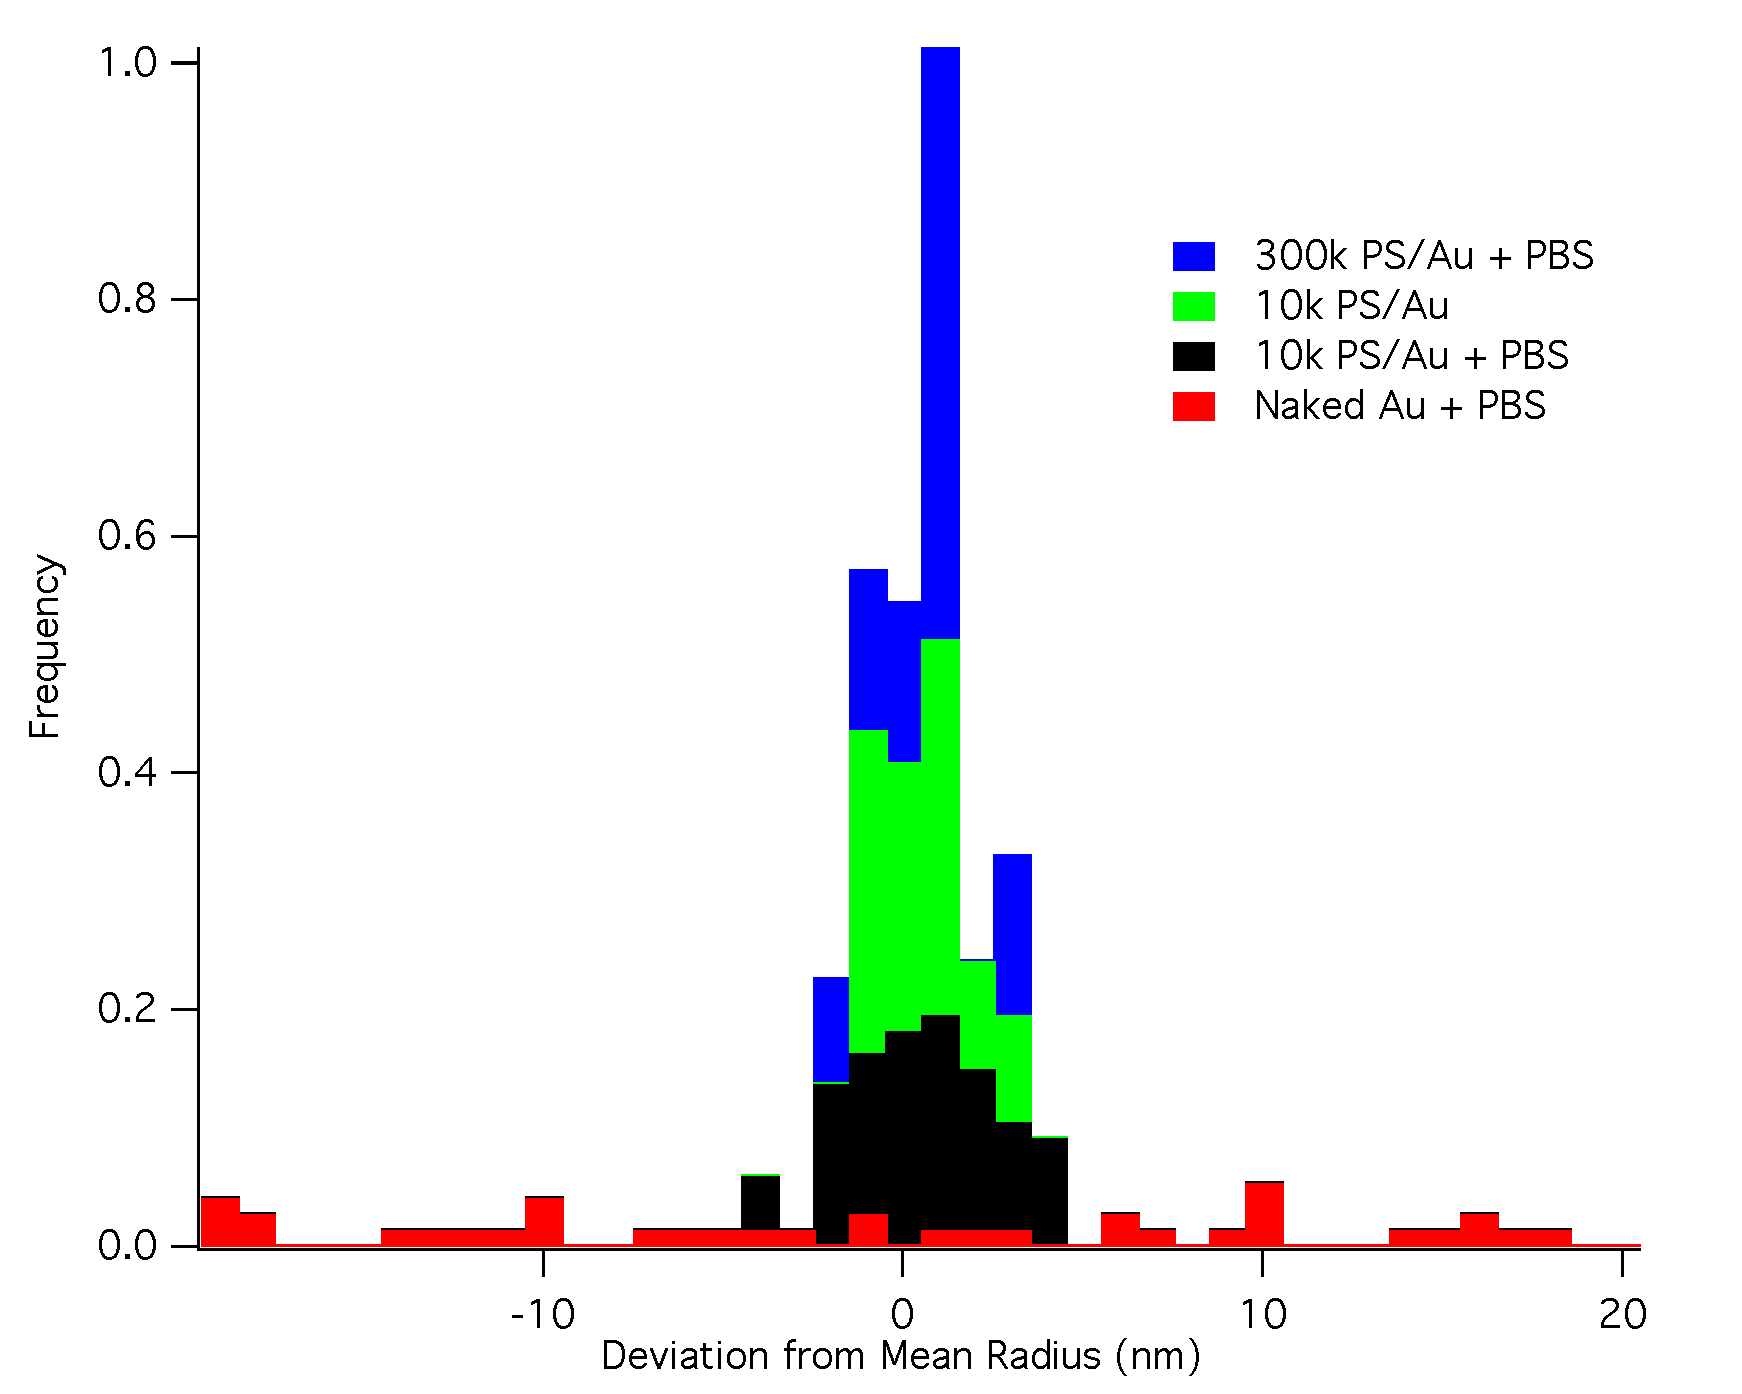
\includegraphics[keepaspectratio,width=5in,height=0.75\textheight]{RadiusHistPBS.pdf}
\caption{Stacked histograms of differing concentrations of Au-PS with and without PBS. The naked gold is significantly broader than any of the other distributions.}
\label{protection}
\end{figure}



For all but the naked gold, almost all acquisitions are within 3 nm of the mean; this is also true of the 300k PS\slash Au without PBS from the summer of 2010. However, with just 10k 5 kDa PS\slash Au, the width of the distribution barely widens when PBS is added--a stark contrast to the addition of PBS to 300k 1 kDa PS\slash Au. Furthermore, there was a \ensuremath{\sim}15 nm increase in average radius between the 1 kDa PS spheres with and without PBS. In the case of the 10k 5 kDa PS\slash Au, the difference in average radius was negligible: 0.09 nm.

From observing the lack of change in both average radius and the change in radial distribution when using the 5 kDa PEG-SH, it is clear that the 5 kDa PEG-SH fully protects the Au nanospheres against capping agent neutralization. There is, however, a noticeable difference between the 10k and 300k PS\slash Au samples; the 300k is slightly narrower, indicating that it offers slightly more protection, consistent with the 300k PS\slash Au solution being on the plateau while the 10k PS\slash Au is still on the rising part of the titration curve.
\newpage
\chapter{Results of the Full Protocol}
\label{resultsofthefullprotocol}

Several fully labeled and protected nanosphere samples were created during the '11--'12 year. The protocol used was adapted from Oliver Hoidn and Perry Ellis's report~\citep{hoidnellis}, using 2,000 antibodies per Au nanosphere and the curve-elbow value 10,000 PEG-SH molecules per Au nanosphere. Detailed documentation of the PEGylation protocol can be found in \autoref{ThePEGylationProtocol}.

The progress of the protocol was monitored by a DLS radius measurement at five or six stages:

\begin{enumerate}
\item Immediately after the addition of the OPAb

\item 24 hours after the addition of the OPAb

\item Immediately after the addition of the PEG-SH

\item 24 hours after the addition of the PEG-SH

\item After dilution with equal parts PBS, to check for protection

\item (For most but not all samples) 48 hours after the addition of PEG-SH

\end{enumerate}

The results of these measurements are shown in \autoref{fullprotocol}. The data shows an immediate increase of 6--8 nm upon the addition of the OPAb, followed by slight ($<$0.1 nm) gains after 24 hours of incubation. AP124F is an IgG antibody and has dimensions of approximately $14.5\mathrm{\,nm}\times8.5\mathrm{\,nm}\times4.0\mathrm{\,nm}$~\citep{antibodylength} as shown in \autoref{iggstructure};
since the NHS replacement can occur on any lysine or N terminus (of which there are several), a 6--8 nm increase in radius is reasonable when all spatial orientations are taken into account.

\begin{figure}[htbp]
\centering
\includegraphics[keepaspectratio,width=\textwidth,height=0.75\textheight]{2011DecPEGylation.pdf}
\caption{Plot of hydrodynamic radii of multiple solutions at each step in the protocol. NOTE: PLACEHOLDER UNTIL I COLLATE ALL THE DATA.}
\label{fullprotocol}
\end{figure}



\begin{figure}[htbp]
\centering
\includegraphics[keepaspectratio,width=3in,height=0.75\textheight]{iggstructure.pdf}
\caption{Structural dimensions of an IgG antibody. From ~\citep{antibodylength}.}
\label{iggstructure}
\end{figure}




Additional analysis can be performed by using the same number estimation as in \autoref{additionofpeg-shtonanospheres}. An OPAb conjugate should have a volume of
\[V=V_{\mathrm{PEG}}+V_{\mathrm{Ab}}=\frac{2.1\mathrm{kDa}}{1.11\frac{\mathrm g}{\mathrm cm^3}}+\frac{160\mathrm{kDa}}{1.35\frac{\mathrm g}{\mathrm cm^3}}=200\,\mathrm{nm}^3\]
Examining the hydrodynamic volume change after the addition of PEG-SH, this corresponds to
\[\frac{4}{3}\pi[(58\mathrm{\,nm})^3-(51.5\mathrm{\,nm})^3]/\frac{200\,\mathrm{nm}^3}{OPAb}=1230\mathrm{\ OPAb}\]
However, this may be an over-estimate, as the 1.35 $\mathrm{\frac{g}{cm^3}}$ density is for the crystalline state of protein~\citep{proteindensity}; the actual effective volume of the OPAb in solution may be larger. Further uncertainty is introduced by the complexity of the diffusion of an Au nanosphere with over 1000 OPAb molecules attached to it. Therefore, this calculation serves primarily as an order-of-magnitude check; in that sense, 1230 OPAb\slash Au compares quite favorably to the 2000 OPAb\slash Au in solution.

We can again perform a calculation of effective footprint: \[A_{\mathrm{OPAb}}=\frac{4\pi(51.5\mathrm{\,nm})^2/\mathrm{Au}}{1230\mathrm{\frac{OPAb}{Au}}}=27.1\,\frac{\mathrm{nm}^2}{\mathrm{OPAb}}\]
This is considerably larger than the effective width of the PEG-SH, indicating that the OPAb molecules on the nanosphere sterically hinder other OPAb molecules from forming thiol bonds with the nanosphere surface. Since the binding mechanism between the PEG chain and the gold surface is the same, this means that there is likely additional room for thiol bonds on the surface, which means that that the PEG-SH should fill in gaps on the surface of the sphere.

Performing the same volumetric analysis on the change in radius from OPAb-Au to OPAb-Au-PS, we see that the number of PS molecules bound to the OPAb-Au is approximately
\[\frac{4}{3}\pi[(59\mathrm{\,nm})^3-(58\mathrm{\,nm})^3]/\frac{7.5\,\mathrm{nm}^3}{PS}=5730\mathrm{\ PS}.\]
This number is the right order of magnitude, given that 10,000 PS\slash Au were added, and only the gaps on the surface are expected to be filled.

The addition of PEG-SH brings the total number of thiol bonded PEG chains on the Au nanosphere surface to approximately 7,000. Though that is not quite the number of PEG-SH molecules that demonstrated protection in Ch.\autoref{additionofpeg-shtonanospheres}, the combination of the 7,000 PEG chains and the antibodies clearly protected the spheres from agglomeration. This is evidenced by the lack of radius increase when the fully labeled and protected nanospheres are diluted with an equal volume of commercial PBS solution, as shown in \autoref{fullprotocol}. Since the radial growth of the spheres matched its predicted behavior fairly well, the decision was made to progress to useing the nanospheres to label a cell culture monolayer.

\newpage
\chapter{Results of the 6 March Labeling Session}
\label{resultsofthe6marchlabelingsession}

With the PEGylation process fully optimized, we took the first step towards immunolabeling a full 3D artificial cornea, namely immunolabeling of a monolayer of cells on a microscope coverslip. The cells used were human dermal fibroblasts (HDFs) that express $\alpha5\beta1$-integrin, the same surface protein that we are targeting on the corneal cells. Performing immunolabeling on the monolayer allows assessment of the efficacy of the indirect immunolabeling process only, disregarding the collagen and removing the financial and temporal costs of building a complete corneal construct.

\section{Structure of the Immunolabeling Experiment}
\label{structureoftheimmunolabelingexperiment}

Several different preparations of cells were used to determine the efficacy of the immunolabeling process. Each of them adds one or more key components of the process, which should yield very little increase in the scattering contrast until the full labeling system is assembled. The 6 preparations and their expected outcomes are described in \autoref{tab:6MarchPrepTable}.

The cells were prepared according to the procedure found in \autoref{The6MarchImmunolabelingProtocol}; in brief, the procedure is

\begin{enumerate}
\item Fix cells with paraformaldehyde

\item Permeabilize with Triton-X

\item Label the nuclei with Sytox Green and the actin filaments with phalloidin (fluorescent stains); simultaneously perform immunoblocking with goat serum.

\item Add primary antibody if appropriate for a given preparation

\item Add secondary labeler (if any)

\end{enumerate}

In between each stage, the sample is washed to remove residues of the previously applied label. Each preparation had three different samples (except for the 2Au preparation, which unfortunately had only two) to minimize intrinsic variation during inter-preparation comparison. After labeling, each sample was imaged in three different places with the confocal microscope, using both fluorescence and backscattering modes, and then each sample was imaged at five different $500\,\mu\mathrm{m}\,\times\,500\,\mu\mathrm{m}$ field of view locations with the OCM (except for 2Au, for which each sample was sampled at 10 different locations).

\rowcolors{1}{}{lightgray} 
\begin{table}[hb]
\caption{Description of the six preparations used in the 6 March immunolabeling experiment; each preparation is described by whether the primary antibody (MAB1999) was added, what secondary labeler (AP124F, AP124F PEGylated to Au nanospheres, or naked Au nanospheres) was added, and whether or not an increase was expected in backscattering or fluorescence.}
\begin{minipage}{\linewidth}
\setlength{\tymax}{0.5\linewidth}
\centering
\small
\begin{tabular}{lp{2cm}p{2cm}p{2cm}p{2cm}} \toprule
Preparation Name&Primary Antibody?&Secondary Labeler?&+Scattering Expected?&+Fluorescence Expected?\\
\midrule
Cells Only&No&No&No&No\\
2 only&No&Secondary Ab&No&No\\
1--2&Yes&Secondary Ab&No&Yes\\
2Au&No&OPAb-Au-PS&No&No\\
1--2Au&Yes&OPAb-Au-PS&Yes&Yes\\
Au&No&Naked Au&Yes but non-specific&No\\

\bottomrule

\end{tabular}
\end{minipage}
\label{tab:6MarchPrepTable}
\end{table}

The first preparation is just cells, grown on a coverslip. In the confocal microscope, a Zeiss LSM 510, we expect to see green fluorescence in the shape of the nuclei from the Sytox Green and red fluorescence in the shape of the actin filaments within the cell from the phalloidin. In the OCM, we expect to see backscatter contrast between the cells and the coverslip; however, the amount of backscattering from the cells should be quite low.

The next preparation is cells with the addition of only the secondary antibody, AP124F. The F in the AP124F signifies the presence of a fluorescent marker, specifically a fluorescein isothiocyanate (FITC) molecule which has an emission spectrum peak at 521 nm. Since the AP124F binds specifically to the MAB1999, and no MAB1999 is present on the surface of the cells, all of the AP124F should be washed off. As a result, the 2 only preparation should be identical to the cells only preparation.

The 1-2 preparation, in contrast, has MAB1999 present. The MAB1999 should bind to the integrins on the surface of the cell, and the AP124F should bind to the MAB1999 in turn. This should manifest itself in the confocal microscope as fluorescence signal at 521 nm. The fluorescence should be localized to the integrins, which are situated in streaks at the edges of the cell. As the AP124F and MAB1999 do not increase the backscattering, the OCM images of the 1-2 preparation should be equivalent to the images of unlabeled cells.

The 2Au preparation should behave just like the 2 only preparation: the lack of MAB1999 should mean that the OPAb-Au-PS spheres cannot bind to anything, and should be washed off. This should result in confocal and OCM images equivalent to those of unlabeled cells.

The 1-2Au preparation should show fluorescence in the pattern of integrins for the same reason as the 1-2 preparation. In addition, the 1-2Au preparation should have gold nanoparticles localized to the integrins, increasing the backscattering signal observed in the OCM.

The naked Au nanospheres have no fluorescent marker, so an increase in fluorescence cannot occur. A scattering increase is expected from the application of the naked Au; however, as the naked spheres have no specific binding mechanism, their binding will not be localized. Instead, the naked Au spheres will likely bind to the coverslip and cells in a homogenous manner through van der Waals forces.

Together, these preparations serve as a set of controls. In the event that the 1-2Au system fails to show any scattering contrast increase, the 2 only and 1-2 only can be used to demonstrate that the AP124F does specifically bind to the MAB1999. This converse is also true: if the 2 only (or 2Au only) show increases in fluorescence or scattering, non-specific binding is occurring, indicating that some part of the PEGylation or labeling process is faulty.

\section{Results of the Immunolabeling Experiment}
\label{resultsoftheimmunolabelingexperiment}

\begin{figure}[p]
\centering
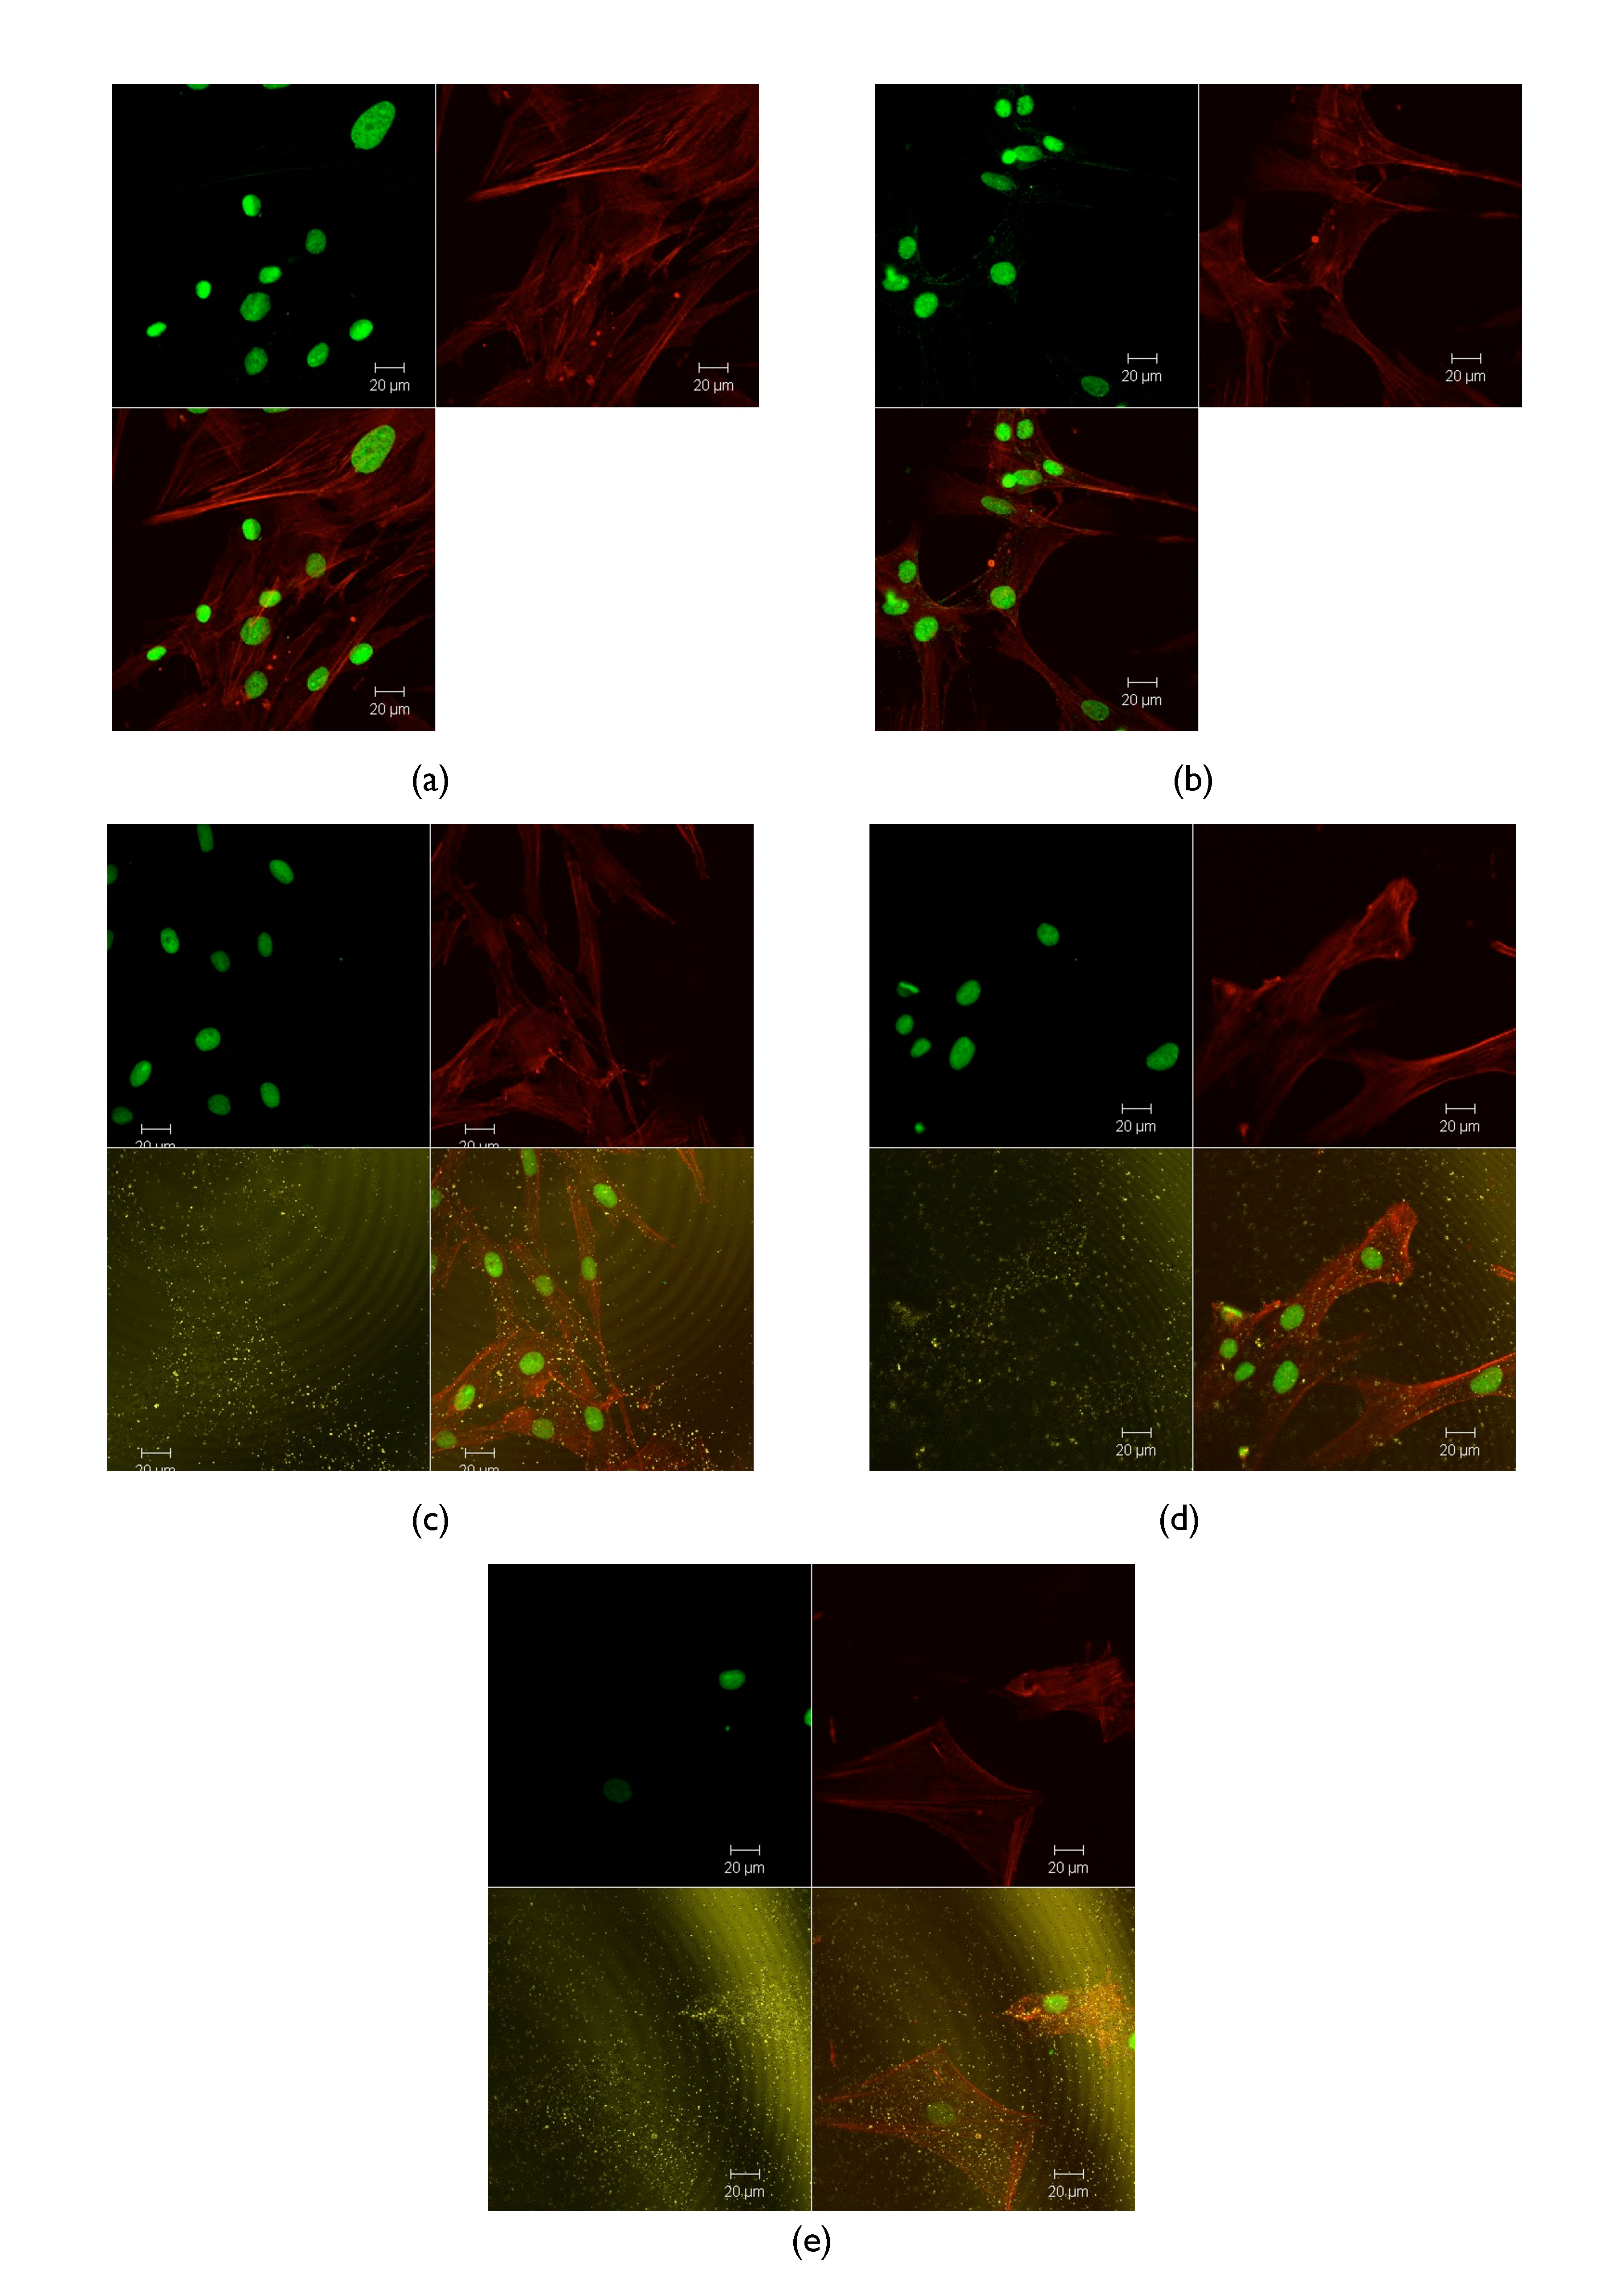
\includegraphics[keepaspectratio,width=\textwidth,height=9in]{ConfocalReps.pdf}
\caption{Confocal images of labeled preparations. Each image is a split view, showing Sytox and AP124F fluorescence (top left), phalloidin fluorescence (top right), backscattered light (c--e only; bottom left), and the composite view (bottom left, a and b; bottom right, c--e). Images correspond to preparations: (a) 2 only; (b) 1--2; (c) 1--2Au; (d) 2Au; (e) Au.}
\label{confocalcollage}
\end{figure}

\begin{figure}[p]
\centering
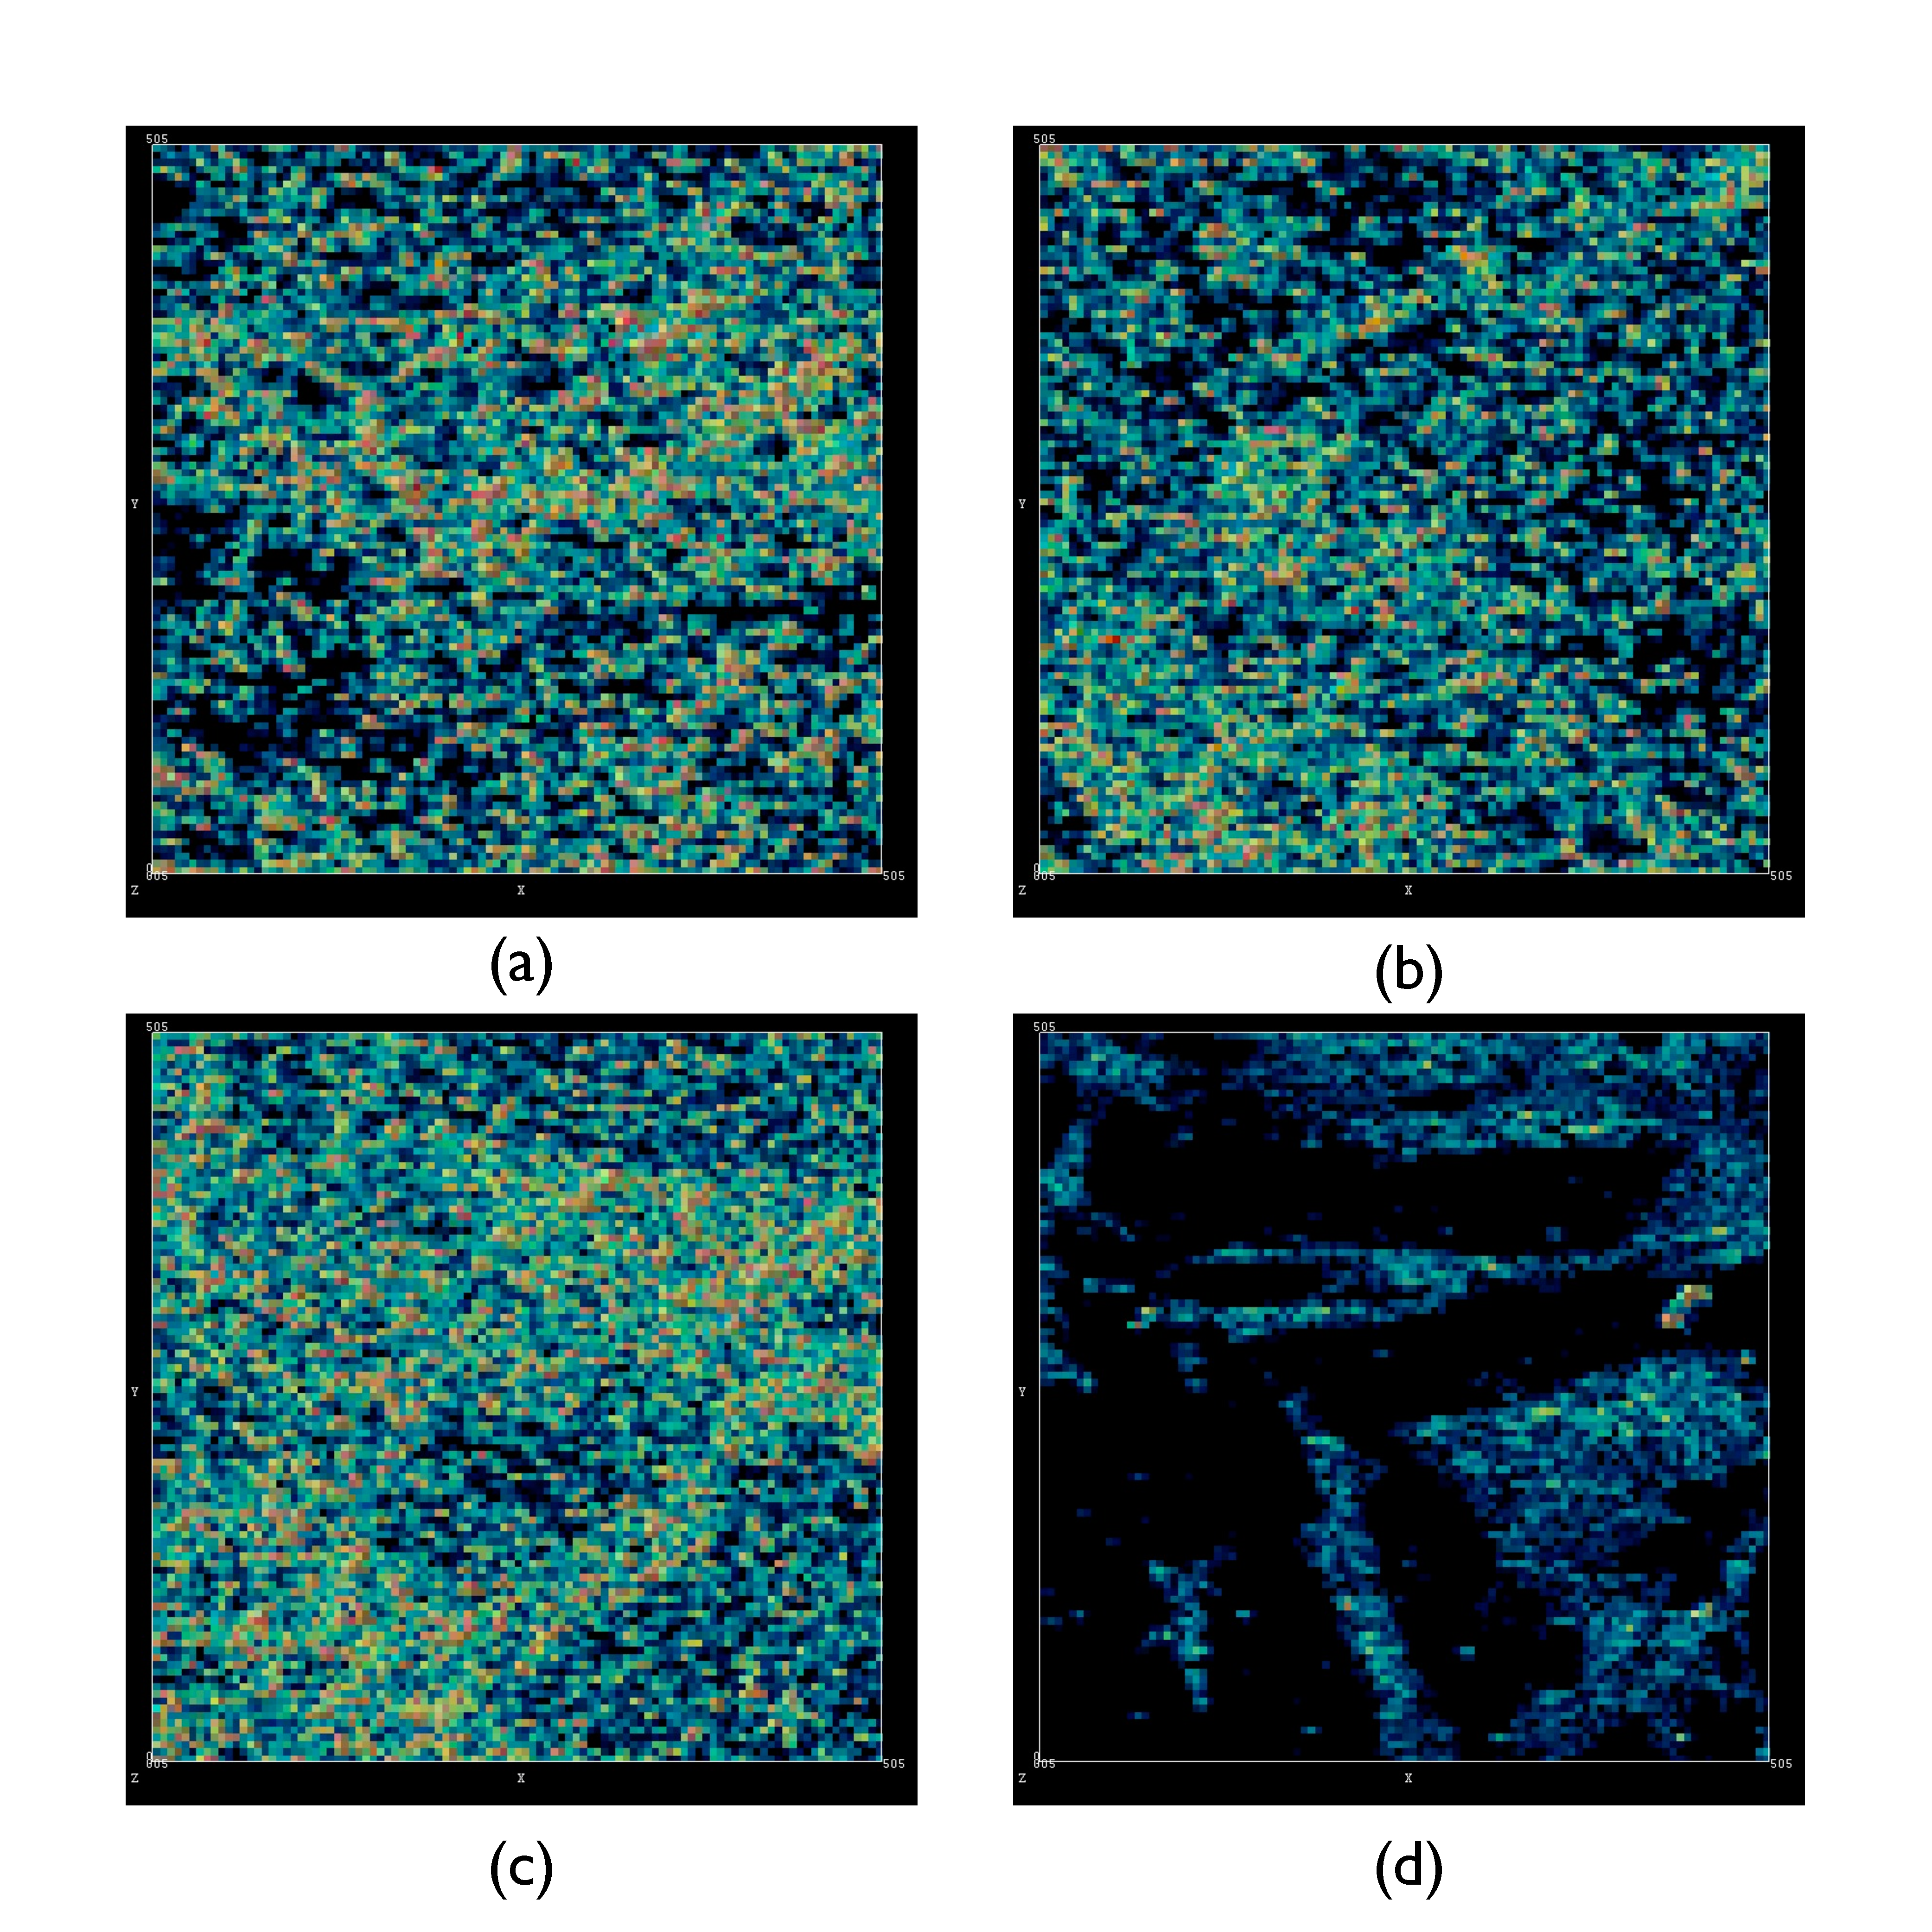
\includegraphics[keepaspectratio,width=\textwidth,height=0.75\textheight]{6marocmreprimages.pdf}
\caption{OCM images of labeled preparations. Images correspond to preparations: (a) 1--2Au; (b) 2Au; (c) Au; (d) Cells only.}
\label{marocmcollage}
\end{figure}

Representative confocal images for each labeled sample are shown in \autoref{confocalcollage}. Examining the between the 2 only and 1--2 confocal images reveals trails of green dots away from the nucleus only in the 1--2 sample; this is the expected pattern of labeled integrins. The appearance of stained integrins in only the 1--2 preparation indicates that both the primary and secondary antibodies bind only to the integrin and primary antibody, respectively. The samples with gold, however, are not as encouraging. Appearance of distinguishable cellular features in the back-reflectance channel indicates that the gold spheres bind to the cells--and to the coverslip--regardless of the presence of either the primary or secondary antibody. Nevertheless, cellular features are more easily distinguished in the 2Au samples, and most easily in the 1--2Au sample. This seems to indicate that some specific binding is occurring, but that a large amount of nonspecific binding is occurring as well.

Representative OCM images for the preparations labeled with gold as well as unlabeled cells are shown in \autoref{marocmcollage}. Clearly, all three gold-labeled preparations show a significant increase in scattering compared to the unlabeled cells. However, as in the confocal images, the Au and 2Au preparations show a strong increase in scattering, and allow for cellular features to be distinguished. Also correlated with the confocal images is the ease with which cellular features can be distinguished: the images from the Au preparation all have a very strong homogenous background, making it harder to discern the features, and in general the cellular features of the 1--2Au more easily distinguishable than those of the 2Au.

\begin{figure}[htb]
\centering
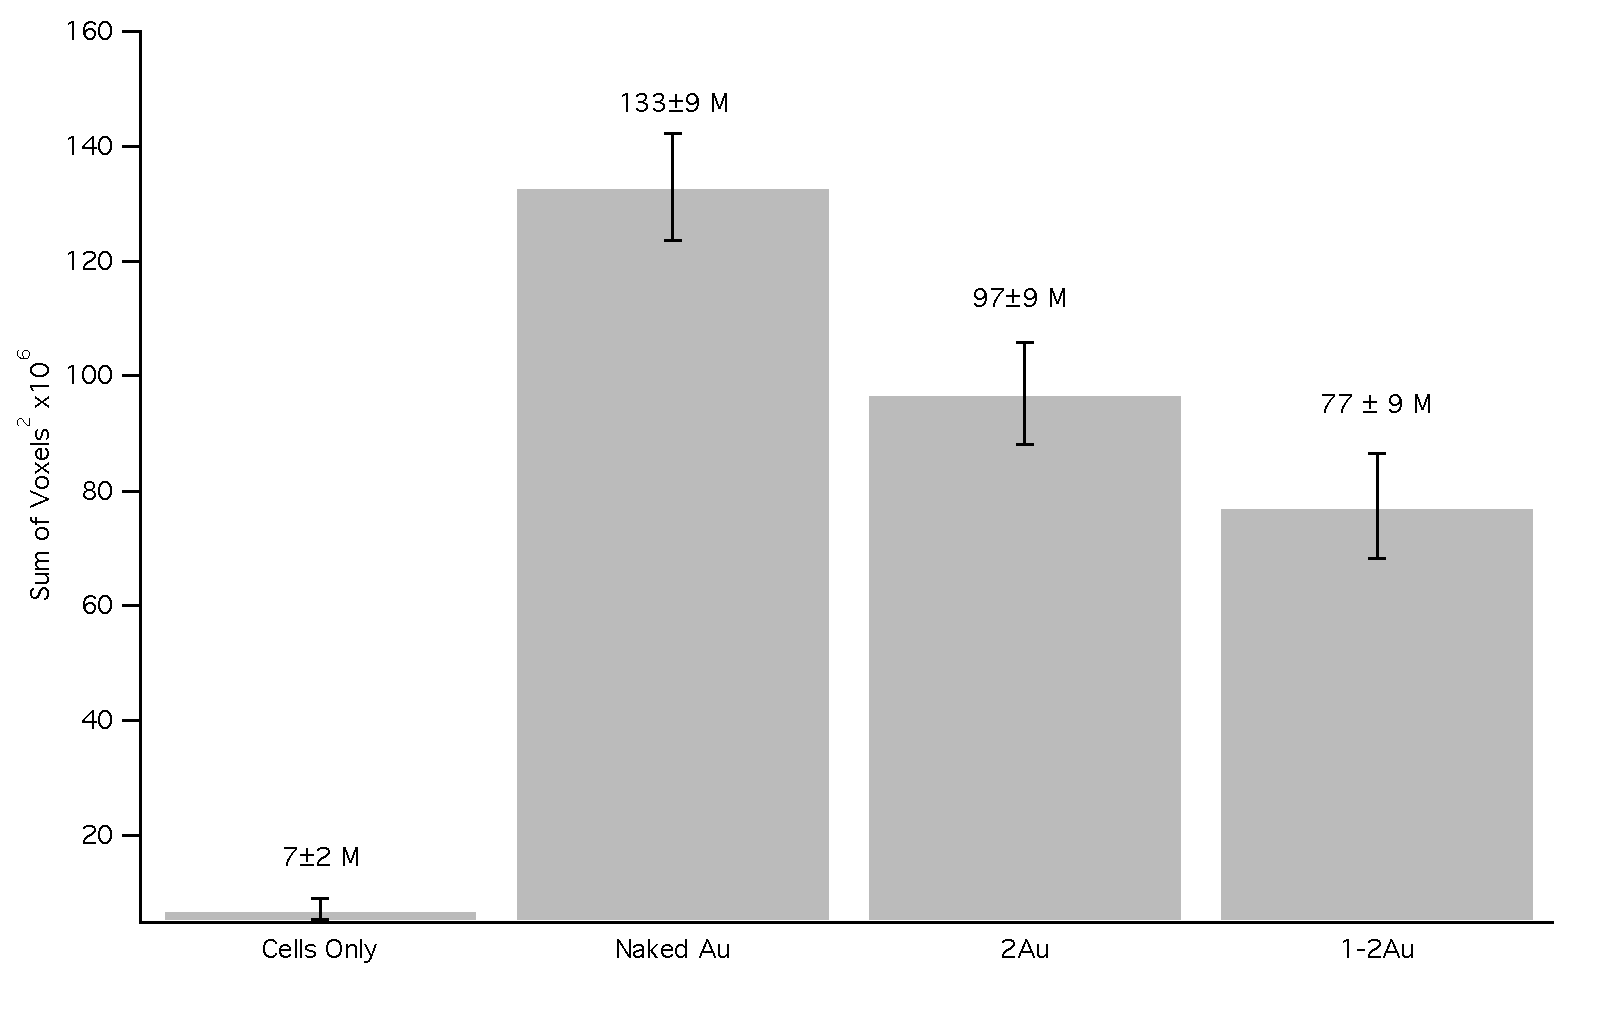
\includegraphics[keepaspectratio,width=\textwidth,height=0.75\textheight]{6marSOSgraph.pdf}
\caption{Sum of OCM voxel values squared for gold-labeled preparations and unlabeled cells; the sum of voxel values squared is a measure of the amount of backscattering from the field of view. Values are formed by taking the mean and standard error of sum of voxel values squared for each image corresponding to a given preparation.}
\label{marsosgraph}
\end{figure}


To quantify the amount of scattering increase, the sum of squares of the values of each voxel was tabulated for each OCM image. The mean and standard error of all the images from a given preparation were then calculated; those results are shown in \autoref{marsosgraph}. The increase in scattering in all three gold-labeled samples is shown quantitatively by comparing their sum of voxel values squared to that of the unlabeled cells. Among the gold-labeled samples themselves, the amount of scattering increase was the opposite of expected: the Au had the most scattering, then 2Au, then 1--2Au. However, the 2Au and 1--2Au samples are statistically indistinguishable.

The high amount of nonspecific binding was puzzling, and two hypotheses were put forth to explain the results of the labeling experiment. One possibility is that all of the spheres, especially the naked Au, bound to the cells via van der Waals forces. Because the naked Au has no dielectric material (protein) separating it from whatever surface it comes in contact with, the strength of van der Waals forces will likely be much larger for the naked Au than for the 2Au. The second possibility concerns the use of Triton-X, a permeabilizing agent. Triton-X is used to permeabilize the cells so that the Sytox Green and phalloidin stains can diffuse inside the cell and stain the nucleus and actin cytoskeleton, respectively. As a result, it was possible that the pores created by permeabilization of the cells allowed Au and 2Au to diffuse into the cell, but once in the cell, the gold nanospheres could not be removed by the washing process, leading to nonspecific contrast enhancement from nanoparticles inside the cell rather than on its surface. Furthermore, noting the strong background in some of the OCM images, there was some concern regarding the binding of the nanospheres to the coverslip surface itself. These concerns (van der Waals, permeabilization, and coverslip binding) led to a second round of immunolabeling experiments being performed on 3 April.
\newpage
\chapter{Results of the 3 April Labeling Session}
\label{resultsofthe3aprillabelingsession}

Given the puzzling results of the immunolabeling experiment performed on 6 March, a second immunolabeling experiment was carried out to answer two lingering questions:
1. Do the naked Au spheres and fully labeled spheres generate nonspecific contrast enhancement by binding to the coverslip?
2. Does permeabilizing the cells with Triton-X so that the cells can be stained with Sytox Green and phalloidin allow the gold nanospheres to diffuse into, but not out of, the cells, leading to nonspecific contrast enhancement?
To address these questions, the gold-labeled preparations from the previous experiments were repeated without permeabilization and two new preparations were added, consisting of coverslips without cells and with gold labeling agents.

\section{Structure of the Immunolabeling Experiment}
\label{structureoftheimmunolabelingexperiment}

The 6 preparations and their expected outcomes are described in the table below.

\rowcolors{1}{}{lightgray} 
\begin{table}[htbp]
\begin{minipage}{\linewidth}
\setlength{\tymax}{0.5\linewidth}
\centering
\small
\begin{tabular}{lccc} \toprule
Preparation Name&1ary Ab?&2ary Labeler?&+Scattering Expected?\\
\midrule
Cells Only&No&No&No\\
Au&No&Naked Au&Yes\\
2Au&No&OPAb-Au-PS&No\\
1--2Au&Yes&OPAb-Au-PS&Yes\\
Coverslip-Au&No&Naked Au&Yes\\
Coverslip--2Au&No&OPAb-Au-PS&No\\

\bottomrule

\end{tabular}
\end{minipage}
\end{table}


Given the results of the previous immunolabeling experiment, the naked Au is expected to increase scattering by binding to the cells and the coverslip via van der Waals forces. Since the OPAb-Au-PS is protected, it should only bind to the cells with the primary antibody; minimal binding should occur between the OPAb-Au-PS and the coverslip. 

The labeling procedure was changed to remove the permeabilization (and the fluorescent stains, as they cannot label without the permeabilization). Full details are in \autoref{The3AprilImmunolabelingProtocol}, but in brief, the procedure was:

\begin{enumerate}
\item Fix cells with paraformaldehyde

\item Add primary antibody if appropriate for a given preparation

\item Add appropriate secondary labeler

\end{enumerate}

Each preparation had three different samples to minimize intrinsic variation during inter-preparation comparison. After labeling, each sample was imaged at five different $500\,\mu\mathrm{m}\,\times\,500\,\mu\mathrm{m}$ field of view locations with the OCM.

\section{Results of the Immunolabeling Experiment}
\label{resultsoftheimmunolabelingexperiment}

Representative images from the OCM are shown in \autoref{aprocmreps}. There is a marked difference between the permeabilized and non-permeabilized preparations (\autoref{marocmcollage}) for the 1--2Au and 2Au preparations. First, cellular features are much more easily distinguished. This is likely due to the fact that the cells were allowed to grow on the cover slips for a shorter period than the previous set of cells, leading to a lower level of cell coverage and thus keeping most cells isolated. This lower cell density is harder to observe in the naked Au image due to the high amount of background from the Au nanospheres binding to the coverslip. The coverslip binding is demonstrated directly by the Coverslip-Au preparation: the binding is fairly homogenous and quite high. The Coverslip--2Au preparation also shows some scatterers present in the volume, though far fewer than the Coverslip-Au preparation. This is further evidence of the successful protection of the gold nanospheres by the PEG-SH and OPAb.

The same sum-of-voxels-squared analysis method was used on this set of images; a chart of those values is in \autoref{aprsos}. There is again clear contrast enhancement and again the naked-Au-labeled cells are quite far above the rest of the samples. This time, however, the scattering from the 2Au-labeled cells is greater than the scattering from the 1--2Au-labeled cells in a statistically significant manner. This is exceptionally puzzling, as it suggests that the presence of primary antibody \emph{decreases} the amount of nonspecific quite considerably, either in conjunction with or instead of increasing the amount of specific binding. Clearly, more work must be done to understand this phenomenon.

\begin{figure}[htbp]
\centering
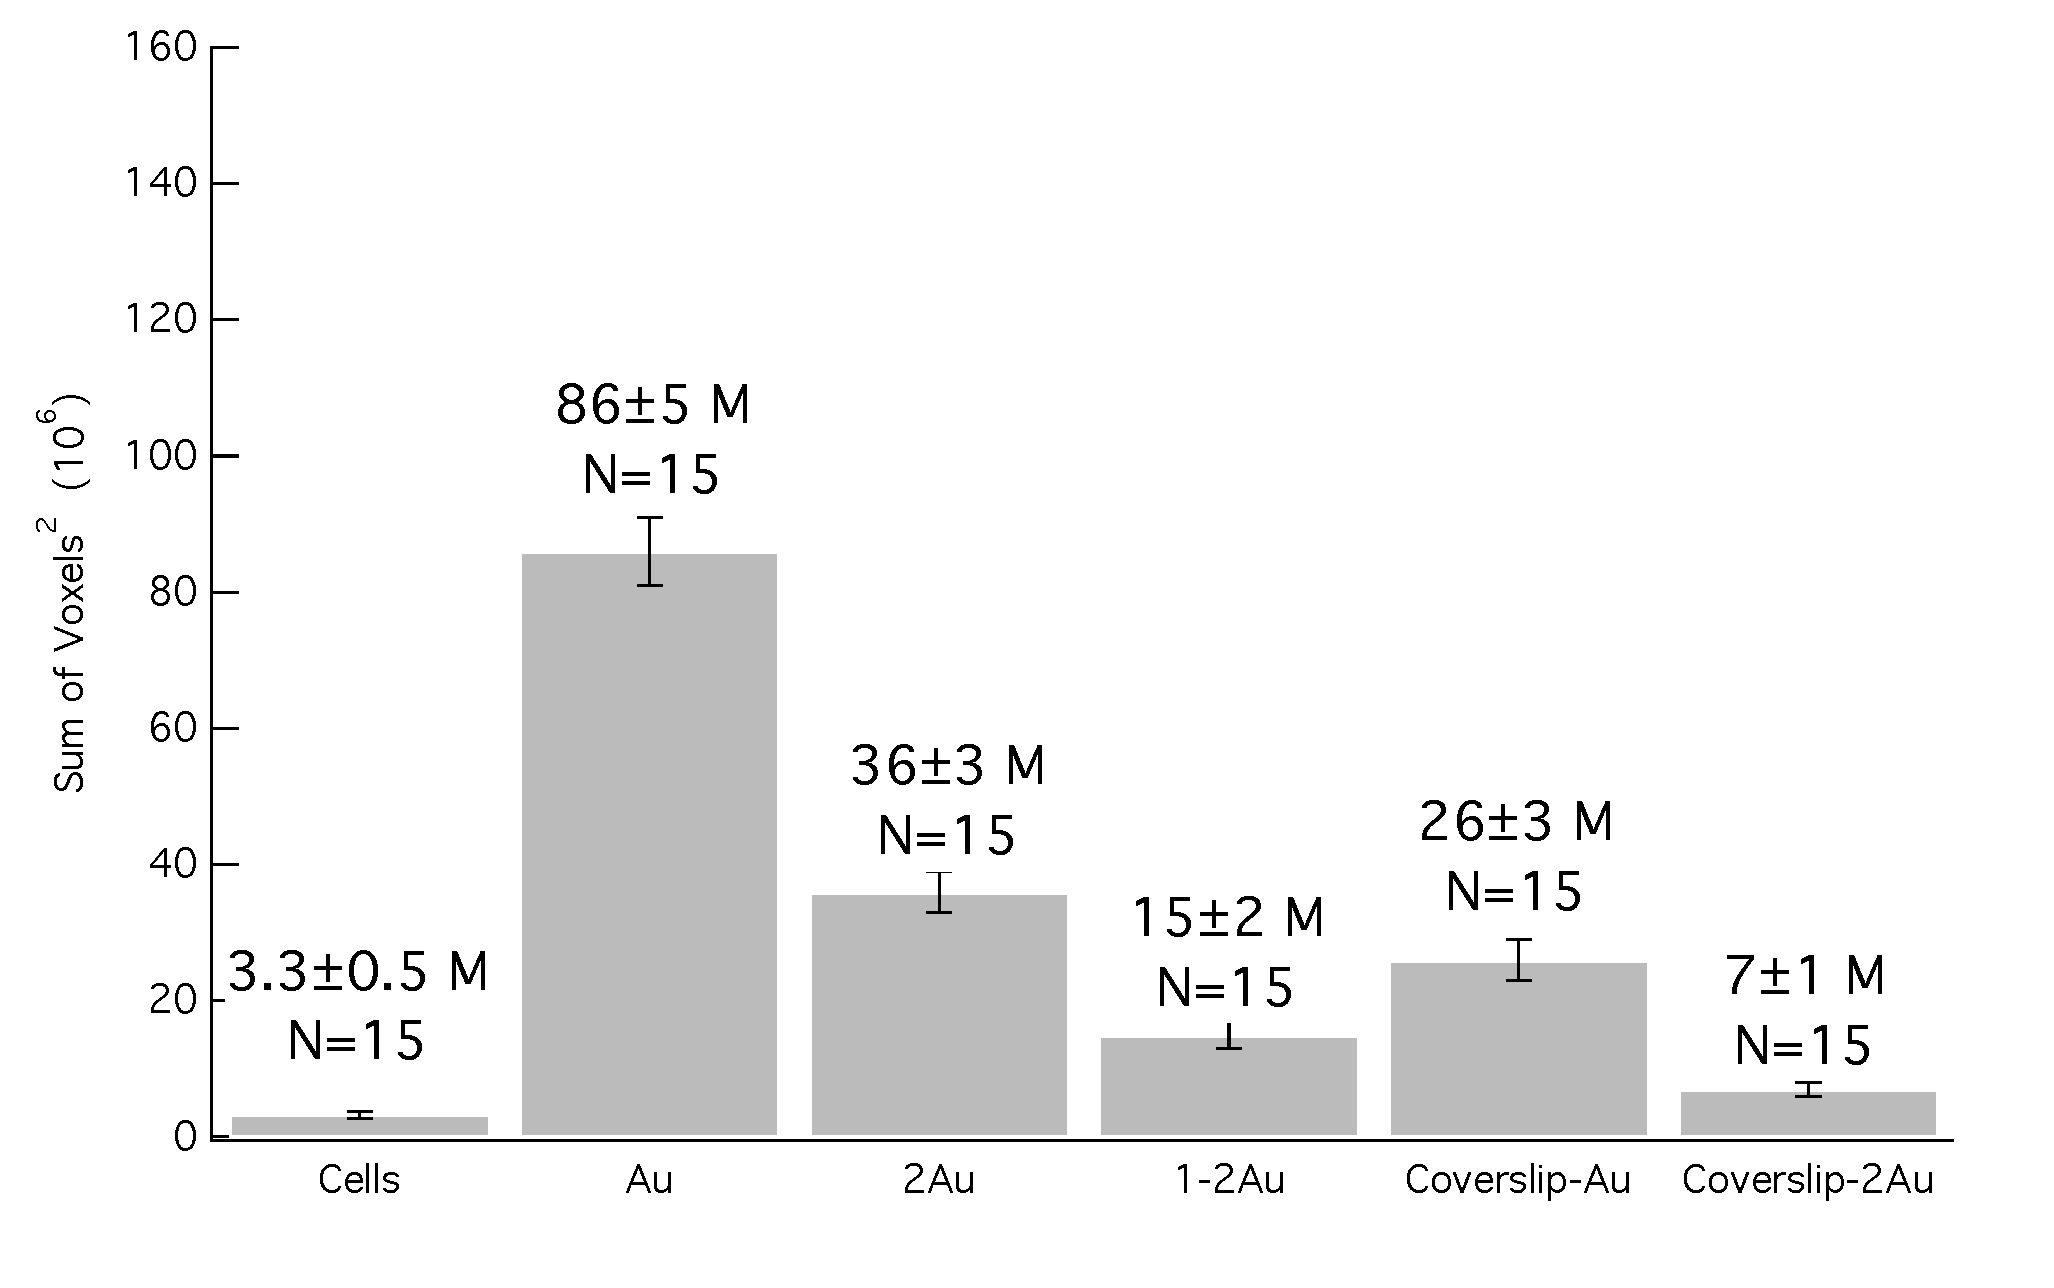
\includegraphics[keepaspectratio,width=\textwidth,height=0.75\textheight]{3aprSOSgraph.pdf}
\caption{Plot of the mean of the sum of voxel values squared for all preparations. Values are formed by taking the mean and standard error of sum of voxel values squared for each image corresponding to a given preparation.}
\label{aprsos}
\end{figure}



\begin{figure}[htbp]
\centering
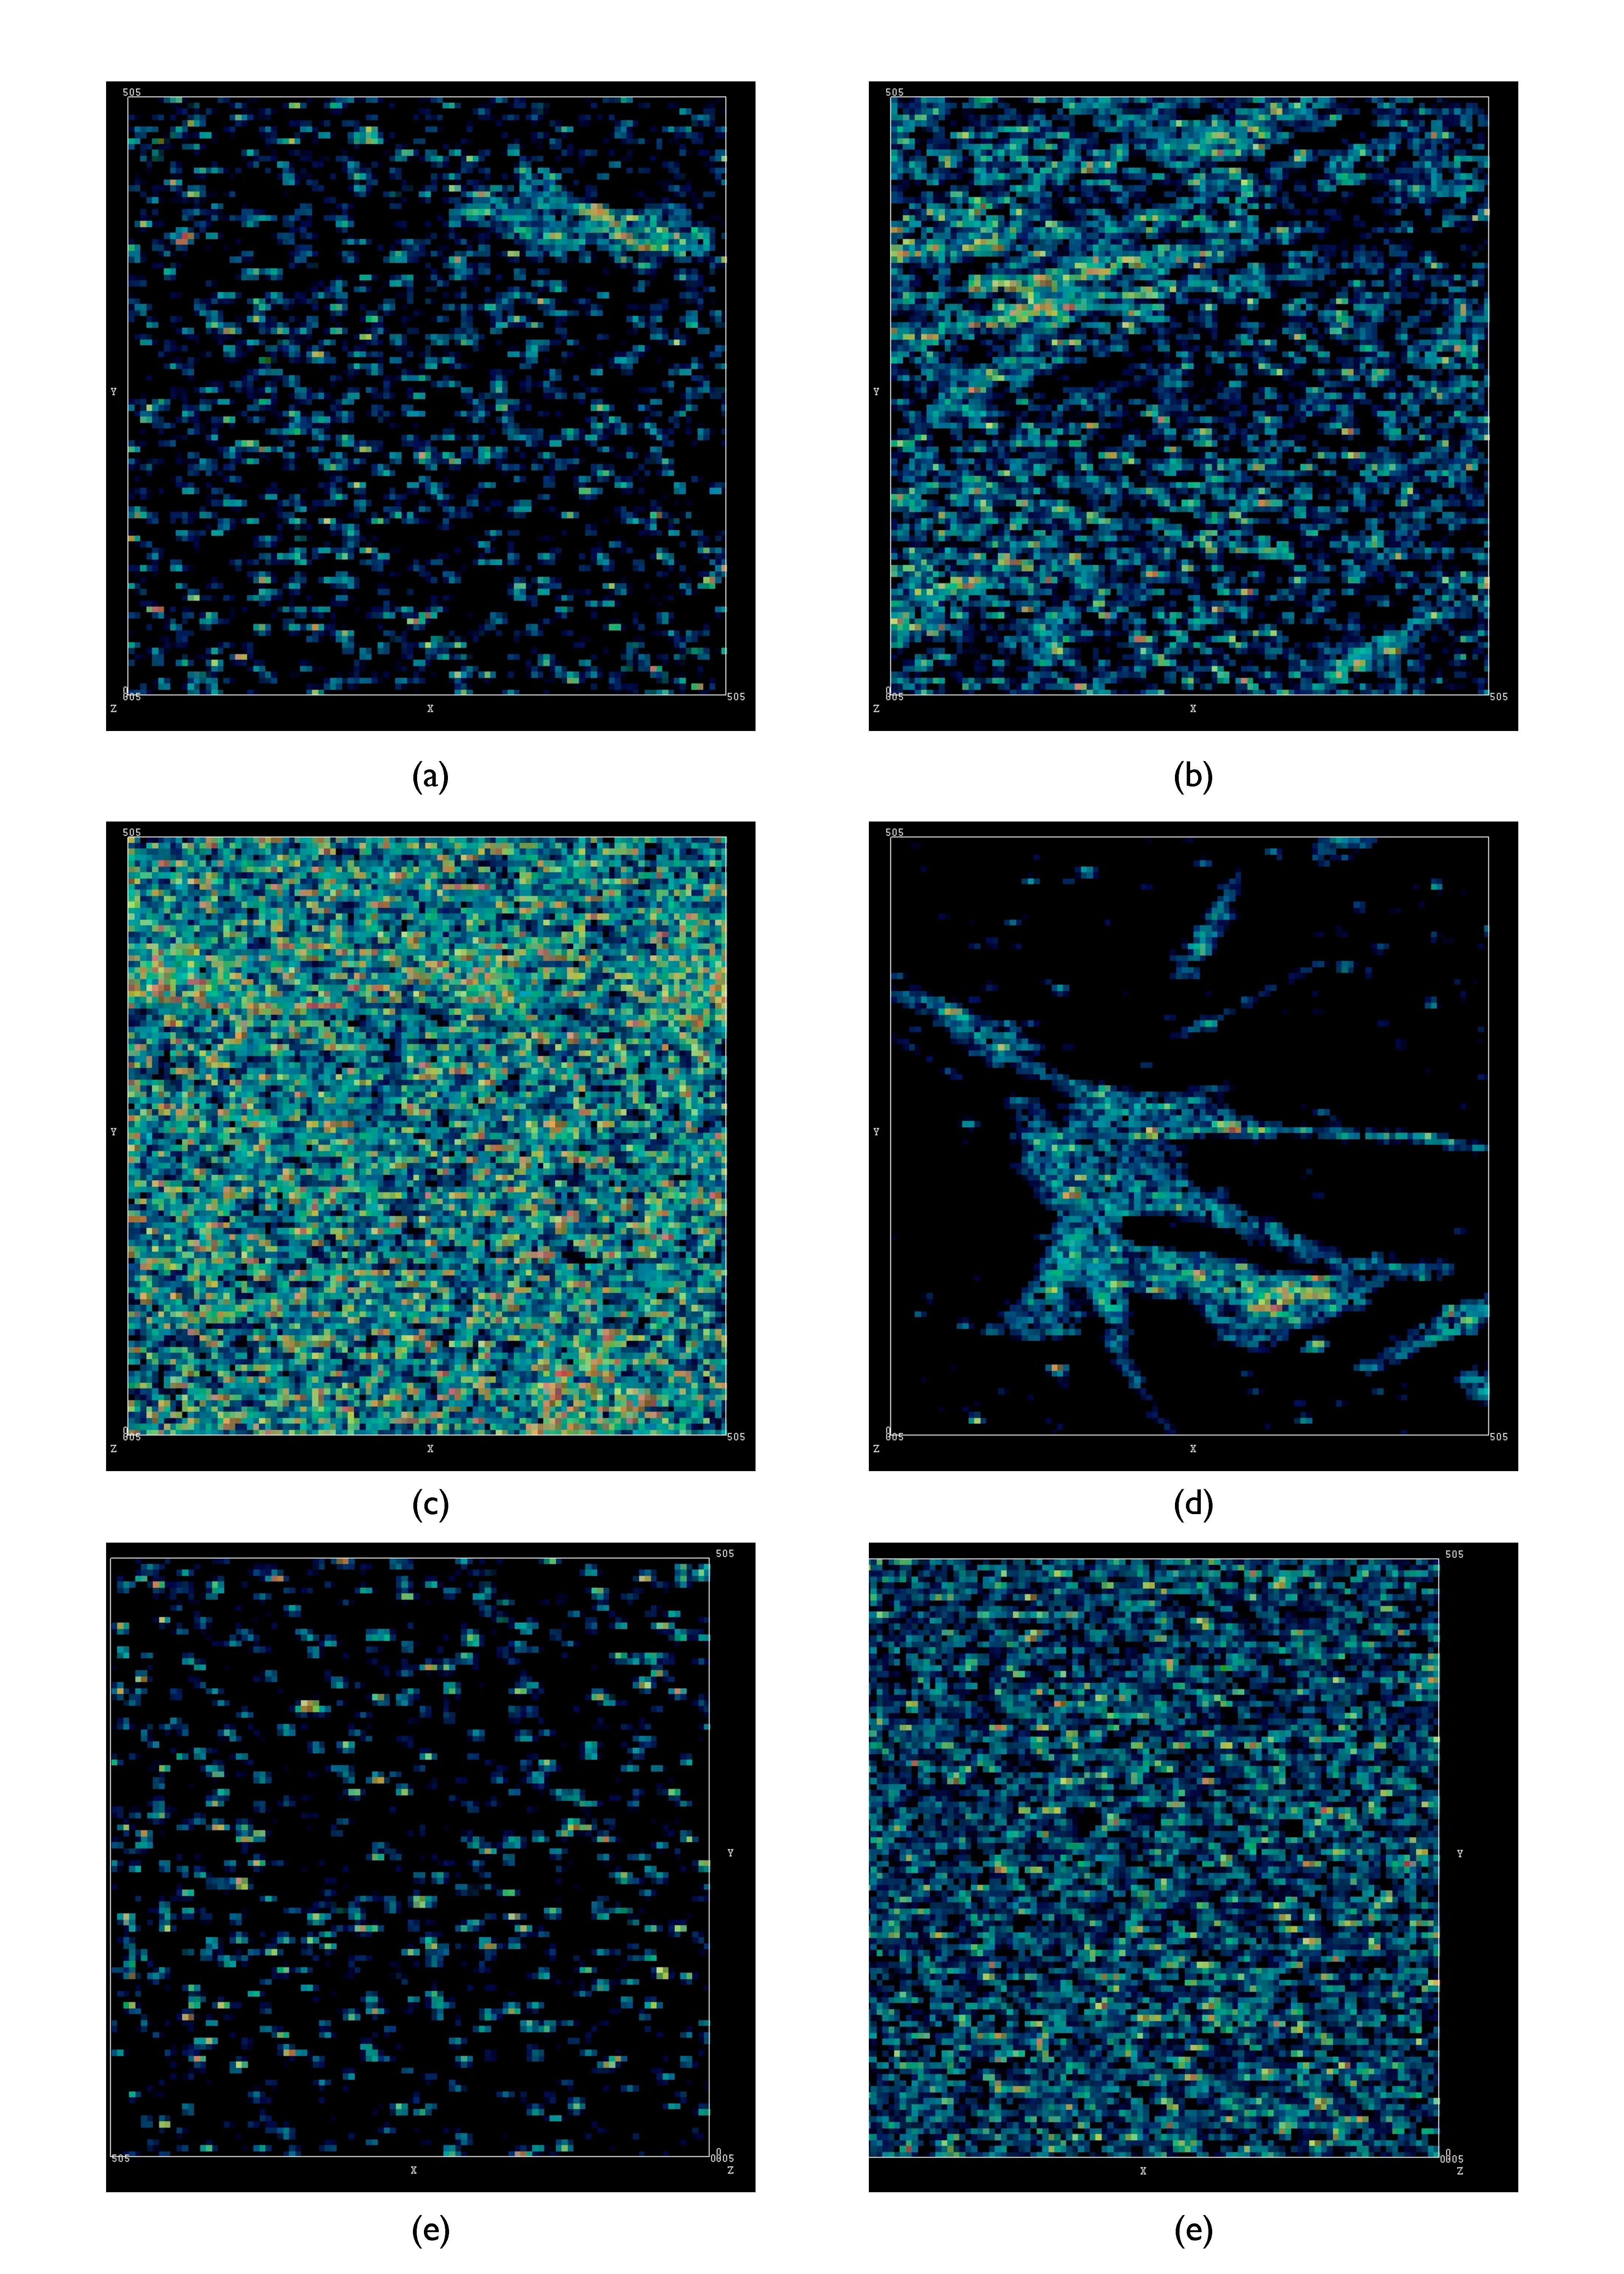
\includegraphics[keepaspectratio,width=\textwidth,height=0.75\textheight]{3aprOCMreps.pdf}
\caption{Representative OCM images of the 6 preparations from the 3 April immunolabeling session. Images correspond to preparations: (a) 1--2Au; (b) 2Au; (c) Au; (d) Cells only; (e) Coverslip--2Au; (f) Coverslip-Au.}
\label{aprocmreps}
\end{figure}




Determining whether or not the permeabilization had an effect is something of a difficult business. Since the cells were at different stages of confluence, the two immunolabeling sessions cannot be compared directly. Rather, some normalization must take into account the different amount of cell coverage. It is not sufficient to simply divide by the scattering from the cells, as that ignores the binding of the spheres to the coverslip. Rather, let us approximate the coverslip and cells as a 2D grid, each pixel of which is either occupied completely by cell or completely by coverslip. Each pixel then contributes, on average, some amount of scattering depending on whether it is cell or coverslip; this amount is determined both by binding affinity and the scattering cross section of the scatterer. The sum of voxels squared, $S_{\mathrm{voxels}^2}$ can then be determined on average as a function of the percent of the viewing region covered by cell, $P$, as
\[S_{\mathrm{voxels}^2}=C_{\mathrm{Coverslip}}(1-P)+C_{\mathrm{Cell}}P\]
where $C_{\mathrm{Coverslip}}\mathrm{\ and\ }C_{\mathrm{Cell}}$ are constants determined by the average scattering from a pixel coverslip or cell labeled with the secondary labeler in question, respectively. We can determine $C_{\mathrm{Coverslip}}$ from the coverslip binding sum of voxels squared; since they are taken at $P=0$, $S_{\mathrm{voxels}^2}=C_{\mathrm{Coverslip}}$. From \autoref{aprsos}, $C_{\mathrm{Coverslip,\,Au}}=2.6\pm0.3\times10^7$ and $C_{\mathrm{Coverslip,\,2Au}}=7\pm1\times10^6$. To determine whether or not reducing the permeabilization had an effect, we need to determine $C_{\mathrm{Coverslip}}$ for Au and 2Au. We now see that we cannot simply divide by the scattering of the cells, which is $C_{\mathrm{Cell,\,Cells}}P$, because that would give
\[S_{\mathrm{norm}}=\frac{C_{\mathrm{Coverslip}}(1/P-1)+C_{\mathrm{Cell}}}{C_{\mathrm{Cell,\,Cells}}}\]
which still has $P$ dependence. However, if we first normalize by subtracting $C_{\mathrm{coverslip}}$, we get
\begin{equation}
S_{\mathrm{norm}}=\frac{S_{\mathrm{voxels}^2}-C_{\mathrm{Coverslip}}}{S_{Cells}}=\frac{-C_{\mathrm{Coverslip}}+C_{\mathrm{Cell}}}{C_{\mathrm{Cell,\,Cells}}}
\label{eq:normalization}
\end{equation}
This is sufficient to perform comparisons between the two immunolabeling sessions, as it does not depend on $P$ at all; $C_{\mathrm{Cell}}$ could be calculated with sufficient image analysis, but generating a large enough dataset to adequately calculate it is beyond the scope of of the studies performed. The results of performing this normalization are shown in \autoref{normalizedsvx2}. For the naked Au the difference is actually the opposite of expected: the permeabilization decreases the amount of scattering per cell coverage; however, the uncertainties on this calculation are quite large, and consequently the difference is statistically consistent with 0. The same hold for the 2Au preparation, though the uncertainties are somewhat smaller and it shows the expected decrease. 1--2Au is the only preparation with a statistically significant difference, and the difference is quite large. Therefore, though there is a large amount of statistical uncertainty, permeabilization does appear to reduce the amount of scattering, which implies that gold spheres are getting inside of the cells. As this is undesirable, and the OCM imaging does not benefit from the fluorescent stains, permeabilization should not be used in future immunolabeling experiments.

\begin{figure}[htbp]
\centering
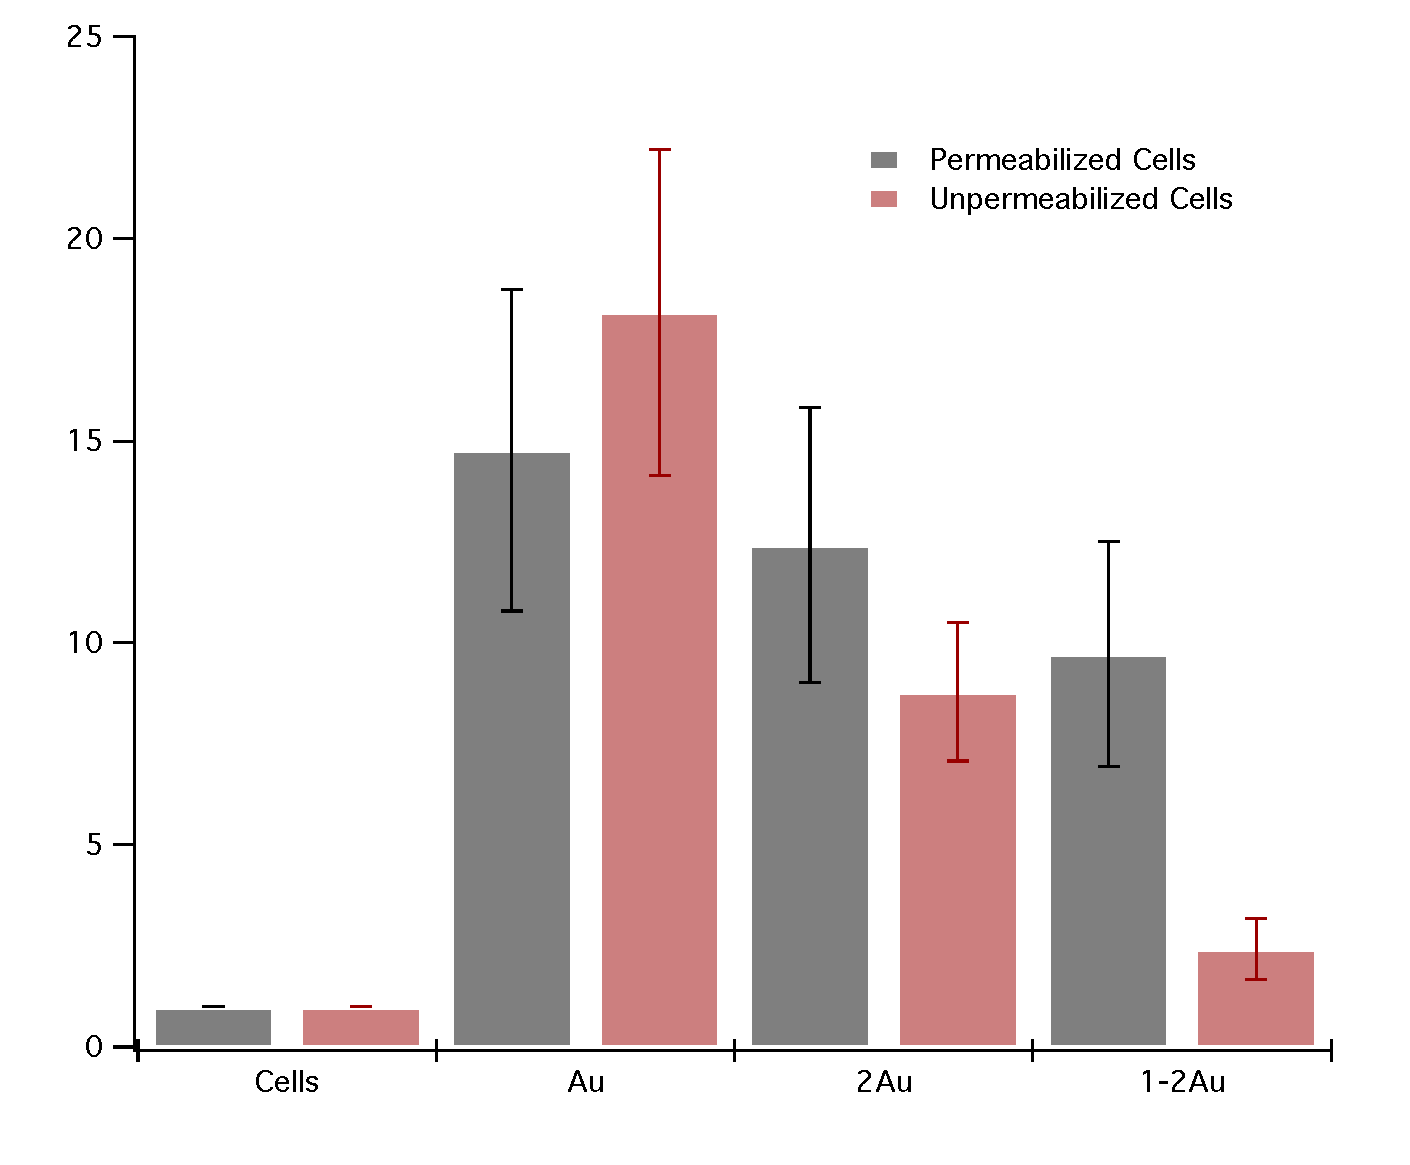
\includegraphics[keepaspectratio,width=\textwidth,height=0.75\textheight]{NormalizedSvx2.pdf}
\caption{Sum of voxel values squared for gold-labeled preparations and cells, normalized using \autoref{eq:normalization}.}
\label{normalizedsvx2}
\end{figure}



As for van der Waals binding, both the Coverslip-Au and the Coverslip--2Au preparations indicate that van der Waals interactions are occurring between the coverslip and the gold, even when it's well-protected by the PEG. Furthermore, there must be strong van der Waals interactions occurring between the cell and the 2Au; though some non-specificity of the secondary antibody is expected, the extent to which the unpermeabilized 2Au preparation displays nonspecific binding to the cell is too large to simply be explained by poor localization of the protein. The high polarizability of the gold creates the potential for strong van der Waals forces, and it may be the case that despite the \ensuremath{\sim}7nm dielectric coating, a strong dipole can be induced in the gold.

\newpage
\chapter{Conclusions and Future Work}
\label{conclusionsandfuturework}

Although the labeling experiments did not produce the hoped-for results of cellularly specific labeling, much progress has been made since the work of Perry Ellis and Oliver Hoidn in the summer of 2010. The PEGylation protocol has been completely optimized, and the spheres seem to be completely protected. In addition, it has been established that permeabilization permits Au nanoparticles to enter the cells, leading to an increase in nonspecific binding.

There are also a number of new and unanswered questions. Most obvious of these is determining why the 2Au preparation experiences greater binding than the 1--2Au preparation. There are two factors that determine the binding: the van der Waals binding, and the specific binding of the secondary antibody to the primary antibody. The van der Waals binding can be calculated numerically if the model of the labeled spheres is drawn up; even without performing the calculations, it is obvious that the 35 nm diameter nanospheres used by the originators of this project would generate far smaller van der Waals forces. Consequently, use of smaller nanospheres may be necessary to reduce the van der Waals binding. The specific binding, to date, has only been measured by the addition of 2Au to primary-labeled cells. However, there is an alternative method by which this could be measured. If OPAb-Au-PS spheres were to be made using the primary antibody (OPAb1-Au-PS) instead of the secondary (OPAb2-Au-PS), then a DLS measurement performed on a mixture of OPAb1-Au-PS and OPAb2-Au-PS should show the spheres agglomerating and precipitating out of solution as the primary- and secondary-labeled spheres form a lattice of sorts. The rate at which this occurs and the final state of the solution should give an approximate measure of the binding strength between the secondary and primary antibodies. It may be the case that the 45 minutes allotted to the 2Au to bind to the primary-labeled integrins is too short to allow for a significant amount of binding; a longer binding period could be used to increase the scattering increase from the 1--2Au preparation. However, this would not explain the large amount of nonspecific binding observed in the 2Au sample; additional investigation of that phenomenon is clearly necessary.


\newpage

\appendix
\chapter{The PEGylation Protocol}
\label{ThePEGylationProtocol}

\begin{enumerate}
\item Create or obtain phosphate buffered Milli-Q (PBM-Q), at least 500 mL.

\begin{enumerate}
\item Based on the work of Ellis and Hoidn \citep{hoidnellis}, the salt concentration of the solution should be 10 mM with a pH of 7.6.

\item To make 500 mL PBM-Q, combine 130 mg $\mathrm{NaH_2PO_4\cdot H_2O}$, 1090 mg $\mathrm{Na_2HPO_4\cdot7H_2O}$, and 500 mL Milli-Q in a 500 mL sealable bottle. The Milli-Q should be measured out in a graduated cylinder.

\end{enumerate}

\item Next, bind the OPSS-PEG-NHS (OPN) to the antibody (Ab). We want approximately a 2:1 ratio of OPN:Ab. The number concentration of the Ab is \[\frac{8.92\times10^{15}\#\mathrm{Ab}}{\mathrm{mL}}=\left(2\mathrm{\frac{mg}{mL}}\right)\left(\frac{6.02\times10^{23}\,\#\mathrm{Ab}}{135 \mathrm{kg}}\right).\] 
Measuring a quantity less than 1 mg of OPN is quite difficult, and we want to use a minimum pipette volume of 5 $\mu$L. Therefore, we will use 6 mg of OPN in 200 mL of PBM-Q. This gives a solution with
\[\frac{8.6\times10^{15}\#\mathrm{OPN}}{\mathrm{mL}}=\left(6/200\mathrm{\frac{mg}{mL}}\right)\left(\frac{6.02\times10^{23}\,\#\mathrm{Ab}}{2.1 \mathrm{kg}}\right).\]
Then, we combine 62.5 $\mu$L PBM-Q, 12.5 $\mu$L Ab, and 25 $\mu$L OPN+PBM-Q solution. Since the concentration of the Ab and OPN are approximately the same, and the volume used of the OPN+PBM-Q solution is double that of the Ab, there should be approximately a 2:1 OPN:Ab ratio. The actual procedure should be as follows:

\begin{enumerate}
\item Fill insulated container with ice.

\item In a 1.5 mL centrifuge tube, combine 62.5 $\mu$L PBM-Q and 12.5 $\mu$L Ab. Put tube in ice.

\item Measure out 200 mL PBM-Q and put in a sealable 250 mL bottle.

\item Measure out 6 mg OPN and add it to the 200 mL PBM-Q.

\item Quickly add 25 $\mu$L OPN+PBM-Q solution to the centrifuge tube, to minimize hydrolysis of the NHS ester.

\item Wait 24 hours for complete binding.

\end{enumerate}

\item Next, bind the OPAb to the Au nanospheres. We want 2000 OPAb\slash Au, and we want 500 mL of labeled spheres. The OPAb concentration is $1.1\times10^{15} \mathrm{\frac{\#OPAb}{mL}}$; therefore, we need
\[\left(500 \mu\mathrm{L} Au\right)\left(5\times10^9\mathrm{\frac{Au}{mL}}\right)\left(2000\mathrm{\frac{OPAb}{Au}}\right)/\left(1.1\times10^{15} \mathrm{\frac{\#OPAb}{mL}}\right)=4.5\mu\mathrm{L\ OPAb}.\] The procedure for this step is:

\begin{enumerate}
\item pH-correct\slash buffer Au solution:

\begin{enumerate}
\item Centrifuge 500 $\mu$L Au at 4200 RPM with soft brake for 10 minutes in a 5417C centrifuge.

\item Remove 2\slash 3 of the supernatant (333 $\mu$L) and replace with PBM-Q, making sure to resuspend the Au solution very well.

\end{enumerate}

\item Add 4.5 $\mu$L OPAb solution made the previous day to the Au solution.

\item Immediately DLS 50 $\mu$L of the OPAb-Au solution.

\item Wait 24 hours for OPAb-Au reaction to complete; again, DLS 50 $\mu$L.

\end{enumerate}

\item The final step of nanoparticle assembly is to add 5 kDa PEG-SH to the OPAb-Au. We want 10000 PEG-SH\slash Au for the 400 mL of remaining OPAb-Au solution.

\begin{enumerate}
\item First, make a PEG-SH+PBM-Q solution. 300 mL PBM-Q and 10 mg 5 kDa PEG-SH gives \[\frac{4\times10^{15}\#\mathrm{PS}}{\mathrm{mL}}=\left(10/300\mathrm{\frac{mg}{mL}}\right)\left(\frac{6.02\times10^{23}\,\#\mathrm{Ab}}{5 \mathrm{kg}}\right).\]

\item To get 10,000 PS\slash Au, we add
\[\left(400 \mu\mathrm{L} \,\mathrm{OPAb-Au}\right)\left(5\times10^9\mathrm{\frac{OPAb-Au}{mL}}\right)\left(10000\mathrm{\frac{PS}{OPAb-Au}}\right)/\left(4\times10^{15} \mathrm{\frac{\#PS}{mL}}\right)=5\mu\mathrm{L\ PS}\]
to the 400 $\mu$L OPAb-solution.

\item DLS 50 $\mu$L OPAb-Au-PS immediately.

\item Wait 24 hours; DLS 50 $\mu$L OPAb-Au-PS.

\end{enumerate}

\item A final, optional step is to check the protection of the fully labeled and protected nanospheres. To do this, obtain a new centrifuge tube and put at least equal volumes (at least 50 $\mu$L) of both OPAb-Au-PS solution and commercial PBS solution. DLS 50 $\mu$L. Radius should be stable if the spheres are protected.

\end{enumerate}


\newpage
\chapter{The 6 March Immunolabeling Protocol}
\label{The6MarchImmunolabelingProtocol}

\rowcolors{1}{}{lightgray}
\begin{table}[htbp]
\begin{minipage}{\linewidth}
\setlength{\tymax}{0.5\linewidth}
\centering
\small
\begin{tabular}{p{4in}rr} \toprule
Action&Volume&Time\tabularnewline
\midrule
Make 10\% goat serum in PBS&&\tabularnewline
Remove media from samples&&\tabularnewline
Cover cells with PBS&500 $\mu$L&\tabularnewline
Fix cells in 4\% Paraformaldehyde (dilute 16\% stock in 1x PBS), shaking, in hood&1 mL&10 min\tabularnewline
Rinse cells with Milli-Q water&500 $\mu$L&2x10 min\tabularnewline
Permeabilize cells in 0.1\% Triton-X (diluted with Milli-Q water) &500 $\mu$L&15 min\tabularnewline
Rinse wells with Milli-Q water twice&500 $\mu$L&2 x\tabularnewline
Incubate with mixture of nuclear stain (Sytox Green 1:2000 dilution) and f-actin stain (rhodamine phalloidin 1:40) diluted in 10\% goat serum at RT in the dark&500 $\mu$L&45 min\tabularnewline
Wash with 10\% goat serum in the dark&500 $\mu$L&3x5 min\tabularnewline
&&\tabularnewline
Label samples with 1:100 Diluted MAB1999 (primary Ab), leave all other samples in goat serum&500 $\mu$L&45 min\tabularnewline
Wash in 10\% goat serum&500 $\mu$L&3x5 min\tabularnewline
&&\tabularnewline
Label relevant samples with undiluted 2-Au, naked Au (or not)&500 $\mu$L&45 min\tabularnewline
Wash in 10\% goat serum&500 $\mu$L&3x5 min\tabularnewline
Leave all other samples in goat serum&&\tabularnewline
&&\tabularnewline
Rinse with PBS&1 mL&1x\tabularnewline

\bottomrule

\end{tabular}
\end{minipage}
\end{table}



\newpage
\chapter{The 3 April Immunolabeling Protocol}
\label{The3AprilImmunolabelingProtocol}

\begin{table}[htbp]
\begin{minipage}{\linewidth}
\setlength{\tymax}{0.5\linewidth}
\centering
\small
\begin{tabular}{p{4in}rr} \toprule
 \rowcolors{1}{}{lightgray} \\
Action&Volume&Time\\
\midrule
Make 10\% goat serum in PBS&&\\
Remove media from samples&&\\
Cover cells with PBS&500 $\mu$L&1 x\\
Fix cells in 4\% Paraformaldehyde (dilute 16\% stock in 1x PBS), shaking, in hood&1 mL&10 min\\
Rinse cells with Milli-Q water, shaker&500 $\mu$L&2x10 min\\
Wash with 10\% goat serum in the dark&500 $\mu$L&45 min\\
&&\\
*Label samples with 1:100 Diluted MAB1999 (primary Ab), leave all other samples in goat serum&500 $\mu$L&45 min\\
Wash in 10\% goat serum&500 $\mu$L&3x5 min\\
&&\\
*Label relevant samples with undiluted 2-Au, naked Au (or not)&500 $\mu$L&45 min\\
Wash in 10\% goat serum&500 $\mu$L&3x5 min\\
*Leave all other samples in goat serum&&\\
&&\\
Rinse with PBS&1 mL&1x\\

\bottomrule

\end{tabular}
\end{minipage}
\end{table}



\newpage

\backmatter

\bibliographystyle{plainnat}

\bibliography{theis}

\end{document}


